\section{Overview}

With a task like Spanish \vsd, where the annotated data is small, a purely
supervised approach has to overcome two challenges: the model overfits the
data, and the model's coverage is small. These were the findings of Chapter
\ref{chapter:supervised}. Chapter \ref{chapter:embeddings} explored a
semi-supervised approach by providing word embeddings as input to a supervised
classifier.

The results of the previous chapter gave evidence in favor of Hypothesis
\label{hyp:embeddings:3}. Recall the hypothesis states that word embeddings had
less tendency to overfit than supervised features. The results served to accept
this hypothesis. However, this improvement in overfitting came with a decrease
in performance: supervised features adapted better to the problem, word
embeddings performed worse. Still the results of word embeddings were
promising, because having less overfitting implies a better performance in
general domain corpora.

The other challenge for this task was coverage. Coverage can be thought of as
the unseen examples, part of a class, that the model can reach (i.e. classify
to the correct class). Examples not in training could add information to the
model that is not integrated in the model yet. One way to add such information
is by adding previously unseen examples to the model. Word embeddings help in
this direction, not by adding new examples to the model, but by adding
information from unlabeled data. With this additional information, the model is
able to cover a wider range of examples.

To increment the model coverage with new examples I explore {\em
self-learning}. This is a semi-supervised technique that expands labeled data
by using the certainty of the model over unlabeled data. It adds new examples
automatically, using a supervised model to label unlabeled examples.  This is a
{\em joint semi-supervised learning} algorithm. This means that labeled and
unlabeled data are used jointly in the process of learning. In contrast, the
approach with word embeddings is {\em disjoint} because embeddings are obtained
independently from the model for \vsd.

The self-learning algorithm works basically as follows. A supervised algorithm
is trained on a seed labeled dataset. Then the obtained model is used to
classify unlabeled examples obtained from a big unlabeled corpus. The certainty
of the algorithm in classification is used to add automatically labeled
examples to the labeled dataset. The algorithm uses this bigger dataset (coming
from both supervised and unsupervised data) to train a new model. This process
is iterated until a stopping criterion is met.

In general terms, self-learning is a simple algorithm that applies a {\em
bootstrap technique} to improve on a supervised model that improves with
unlabeled data. The objective of exploring this technique relies on
incrementing the model coverage as I said before. The underlying assumption is
that the new examples will help the model integrate the information that is
latent on those examples.

However there is a challenge I need to face when coming to train a model using
a self-learning approach. This challenge resides in the imbalance of the
classes in the corpus. If the initial model is biased to classify the instances
as part of the most common class, this error will be dragged by the
self-learning model and will automatically annotate new examples as the most
frequent class just because the original model does so. 

Moreover, in this particular case there is another problem, and that is the
specific domain of the corpus on which the initial model is trained. Recall
that SenSem, the resource I am basing the experiments on, comes from a specific
domain: journalistic. Having a biased domain also affects which classes appear
the most. Thus some classes are the most common in a general domain but this is
not the case for the specific domain as the next examples illustrates:

\begin{example}
  The verb ``llegar'' has 8 different senses in SenSem. Of them, one is ``to
  reach certain height or point''. This sense is not the most common one
  available in the SenSem corpus as it has a few labeled examples in the
  corpus. However in a more broad domain it can be used with a higher
  prevalence than in this domain.
\end{example}

These are the reasons behind studying different techniques in the previous
chapters to avoid overfitting and bias to the most frequent class in the
supervised algorithm. This is important for the self-learning algorithm to
avoid diverging to the most frequent class too quickly and thus not adding
enough useful, diverse information to the model.

This chapter will test the following hypothesis:

\begin{hypothesis}\label{hyp:self-learning}
  The target classes of a model trained on labeled data can be better
  represented by integrating more examples, even if they are automatically
  labeled (and thus contain error and bias). Increasing the number of examples
  to train a model helps to avoid overfitting of the model and improves
  coverage.
\end{hypothesis}

In order to accept or reject such Hypothesis, I divide it in more specific
ones. 

First I make two hypotheses about the general goodness of this approach to
improve upon a mostly supervised approach:

\begin{subhypothesis}\label{hyp:self-learning:1}
  The performance of the model over the held-out test data improves after the
  self-learning algorithm adds new automatically annotated examples.
\end{subhypothesis}

\begin{subhypothesis}\label{hyp:self-learning:2}
  The model obtained in each iteration shows an increase in the average
  certainty to predict the class of unseen examples. 
\end{subhypothesis}

Concerning overfitting, I make the following hypothesis:

\begin{subhypothesis}\label{hyp:self-learning:3}
  Increasing the number of examples helps reducing overfitting.
\end{subhypothesis}

Concerning coverage, I make the following hypothesis: 

\begin{subhypothesis}\label{hyp:self-learning:4}
  The self-learning algorithm increases the number of features associated to
  the model, which is an indicator of an increment in the coverage of the
  model.
\end{subhypothesis} 

Given the initial bias in the distribution of classes and the bias of the
self-learning algorithm to amplify this initial bias and overpopulate a
majority class, the following hypotheses are expected to be rejected:

\begin{subhypothesis}\label{hyp:self-learning:5}
  Self-learning helps improving the performance of the model on each of the
  classes uniformly.
\end{subhypothesis}

\begin{subhypothesis}\label{hyp:self-learning:6}
  The representativity of each class in the dataset is kept through all
  iterations of the algorithm.
\end{subhypothesis}

\begin{subhypothesis}\label{hyp:self-learning:7}
  The coverage of the features is uniformly distributed across classes.
\end{subhypothesis}

These hypotheses will be accepted or rejected using the following layout:

\begin{itemize}
  \item Experiment \ref{exp:self-learning:1} reports the performance of a model
    before and after running the self-learning algorithm. The performance is
    measured by the macro and weighted average F1-score (Metric \ref{met:1}).
    Results shown in Section \ref{sec:self-learning:hyp:1} serve to test and
    mildly reject Hypothesis \ref{hyp:self-learning:1}, that the performance
    over a model on held-out test data improves after the self-learning
    iterations.
  \item Experiment \ref{exp:self-learning:2} shows the certainty the model over
    predicted classes for each iteration of the algorithm. The average of this
    value is what I need to test Hypothesis \ref{hyp:self-learning:2} which
    states that the model has an increase in the average certainty along
    self-learning iterations (Metric \ref{met:5}). The results of this
    experimentation are shown on Section \ref{sec:self-learning:hyp:2} and show
    that certainty is not increased, thus this Hypothesis is rejected.
  \item Experiment \ref{exp:self-learning:3} assesses overfitting by measuring
    the error due to variance of a model trained on one dataset over other
    datasets. To measure this I use the learning curve (Metric \ref{met:3}) I
    already explained in previous chapters. The results of the experiments
    shown in Section \ref{sec:self-learning:hyp:3} serve to mildly reject
    Hypothesis \ref{hyp:self-learning:3} which states that adding new examples
    to the dataset helps to decrease the model tendency to overfit. 
  \item Experiment \ref{exp:self-learning:4} records the number of features a
    model has. This number of features is measured by raw count. Results shown
    in Section \ref{sec:self-learning:hyp:4} serve to accept Hypothesis
    \ref{hyp:self-learning:4} that the self-learning algorithm increases the
    number of features associated to the model.
  \item Experiment \ref{exp:self-learning:1} also serves as the base to test
    Hypothesis \ref{hyp:self-learning:5}, that the self-learning algorithm
    improves the performance of each class uniformly. To test this hypothesis I
    look at the results from a different perspective. Section
    \ref{sec:self-learning:hyp:5} discusses the results regarding this
    hypothesis. This time however I do not use the average of F1-score (Metric
    \ref{met:1}), but rather the F1-score of each class before and after the
    self-learning iteration. Results show that, as expected, the hypothesis is
    rejected.
  \item Experiment \ref{exp:self-learning:5} records the distribution of the
    classes in the training dataset for each of the iterations in the
    self-learning algorithm. This distribution is measured by the proportional
    count of such classes. The results of this experiment measured with the
    metric are displayed in Section \ref{sec:self-learning:hyp:6} and serve to
    reject Hypothesis \ref{hyp:self-learning:6} of the classes being uniformly
    distributed across self-learning iterations.
  \item Experiment \ref{exp:self-learning:4} is also used, measured differently
    this time, to test Hypothesis \ref{hyp:self-learning:7}. The experiment
    collects the number of times a feature and a class co-occur in the training
    dataset. These results are measured by two different metrics. First the raw
    count of features per class. On the other hand I also look into the
    association each class has to each feature. To do this I use the pointwise
    mutual information defined in Metric \ref{met:4}. The results that serve to
    reject the Hypothesis are shown on Section \ref{sec:self-learning:hyp:7}.
\end{itemize}

In Section \ref{sec:self-learning:previous} I revise some previous work done in
self-learning in general and also specifically applied to \vsd. Also I mention
some other semi-supervised methods based on bootstrap techniques.

In Section \ref{sec:self-learning:methodology} I go through the relevant items
that concern to the experimentation done in the chapter. Section
\ref{sec:self-learning:resources} reintroduces the resources I work with in the
experimentation. Most of them were already introduced and I only do a quick
summary with references to the section where the resource is better explained.
Next in Section \ref{sec:self-learning:features} I explain the features and
representations I work with in this chapter, and particularly give some hints
on how to deal with the add of new examples by the model and how this affects
the representation by adding new features as well. Section
\ref{sec:self-learning:algorithm} explains the fine detail of the self-learning
algorithm, including certainty threshold and stopping criterion the algorithm
uses. Finally Sections \ref{sec:self-learning:experiments} and
\ref{sec:self-learning:metrics}, as in previous chapters, lists the experiments
and metrics I use to measure the results respectively.

Section \ref{sec:self-learning:results} reports the results of the experiments
and analyzes them in order to accept or reject the stated hypotheses of the
chapter.

Finally Section \ref{sec:self-learning:conclusions} draws the conclusions of
this chapter, recapitulating the Hypotheses and the implications of accepting
or rejecting them according to the evidence gathered in the results. It states
the shortcomings of the methods explored in this chapter and what I want to
accomplish on the next. It ends by outlining future work.

\section{Relevant Work}\label{sec:self-learning:previous}

As explained in Section \ref{sec:general_background:self-learning}, of Chapter
\ref{chapter:general_background}, self-learning is one of the first approaches
in using a semi-supervised learning technique with quite some time in the
literature \cite{Scudder:2006:PEA:2263254.2267291}. The idea has been applied
in many natural language tasks besides \wsd: subjectiveness in nouns
\cite{Riloff:2003:LSN:1119176.1119180}, dialogue classification
\cite{Maeireizo:2004:CPE:1219044.1219072}.

For self-learning applied to \wsd, the work of Yarowsky \cite{yarowsky-95} to
build a disambiguation model based on the words co-occurring with manually
labeled examples is fundamental in the area. The exploration done in this
chapter takes most of its ideas from this work. Another work is the one by
Mihalcea \cite{mihalcea:2004:CONLL}, on which she explores the different
settings of hyperparameters one can have in the algorithm to improve the
performance of the supervised task.

\section{Methodology}\label{sec:self-learning:methodology}

This chapter explores the self-learning algorithm to expand a supervised model
with unlabeled data annotated automatically based on certainty. The
self-learning algorithm is a {\em wrapper}. This means the self-learning
algorithm does not classify data by itself. It does it by wrapping a supervised
classifier. Then it uses the information the supervised classifier gets from
the data to augment the model.

Recall that independent classifiers are learnt for each lemma. I describe the
methodology in general terms, but I still run one self-learning algorithm model
per each lemma. It is important to keep in mind that evaluation metrics may
obscure differences in performance across lemmas.

\subsection{Resources}\label{sec:self-learning:resources}

Self-learning requires two main resources: a labeled and an unlabeled dataset.
The labeled dataset is the seed of the initial model. From this data the
algorithm bootstraps the iterations. The unlabeled dataset is the source of new
examples to annotate automatically. The experimentation for this chapter is
done only on the Spanish corpora.

Initially I wanted to do a general analysis of the results of \vsd~for all the
available lemmas. However, while working on the analysis, giving a much closer
look to the data, it was concluded the best method was to take some token
lemmas and analyze them with a much closer look to see how the algorithm works
on each of those cases. Besides this, the other reason to do so was to have
some point of comparison when doing active learning in the following chapter as
the availability to manually labeled data was limited.

As token lemmas, I selected a communication verb, originally ``hablar'' was
intended, but there were annotated examples of only one sense, thus
``explicar'' was chosen instead. I also selected ``pensar'', another verb of
the communication class, to observe similarities and differences. Two verbs of
movement were next: ``acceder'' and ``llegar''. Finally two transitive verbs
were selected: ``buscar'' and ``facilitar''.

\subsubsection{SenSem}

The SenSem corpus is used as the annotated seed on which the self-learning
algorithm starts. For more information on this resource please refer to Section
\ref{sec:supervised:sensem}.

The main problem with using SenSem as it is in self-learning is how it is
affected by the algorithm's tendency to diverge to the most frequent class. As
I will show in the results further in this chapter, this is a big problem
regarding self-learning. A first approach I had to follow in order to deal with
this problem was oversampling.

I randomly oversampled the examples of the less frequent classes in order for
the initial (seed) dataset had an equivalent number of examples for each class.
This did not completely fixed the algorithm's tendency to classify everything
as part of the most frequent class, but it did help in smoothing this. If I
used in the experiments the original dataset without oversampling then the
algorithm's drifting was much more quicker. This oversampling had no impact on
the performance of the supervised algorithm (i.e. the classifier trained only
on labeled data) over the test corpus, but did help in the case of the
self-learning iterations to delay the drifting to the most frequent class.

\subsubsection{SBWCE}\label{sec:self-learning:sbwce}.

The unlabeled data source of new instances for the algorithm is the SBWCE.
This resource was already described in Chapter \ref{chapter:embeddings},
Section \ref{sec:embeddings:sbwce}.

Due to time and resources constrains I was not able to use the full resource.
The algorithm takes and classifies the unlabeled data to select the instances.
Then with the full SBWCE dataset each iteration would take a large amount of
time to complete. The solution was to randomly sample a fixed number of
unlabeled sentences for each lemma. For each lemma I chose 1000 unlabeled
sentences and used them as unlabeled data for self-learning.

Once the sentences were selected the corpus is preprocessed to add PoS and
dependency annotations. The preprocessing step is done with Freeling. The key
idea is to have in the unlabeled dataset the same type of information as the
supervised dataset, as described in~\ref{sec:supervised:sensem}. This
information is used to build the hand-crafted features.

\subsection{Features}\label{sec:self-learning:features}

The previous chapter showed that word embeddings are promising but supervised
features still have the best performance. I decided to keep both kinds of
features and compare how each performs on jointly semi-supervised learning
tasks. Parameters for both kinds of representations are the ones with the best
performance in previous chapters.

\subsubsection{Hand-crafted features}\label{sec:self-learning:handcrafted}

For hand-crafted features I use the features described in Chapter
\ref{chapter:supervised}, Section \ref{sec:supervised:features}. 

Recall the whole set of hand-crafted features for the supervised data was
already large even though the labeled dataset was small. When this is done for
unlabeled datasets the amount of features are most likely too big to fit in
memory.

Moreover, the original supervised model of the self-learning algorithm is
trained only on the supervised data. Then it only has the features the
supervised corpus has. These features are not likely to be the only ones
available in the unlabeled dataset.

As most of the classifiers take a fixed size input, having new features from
unlabeled data gives two options: ignore the features or generate a
representation with the features of the whole dataset (i.e. labeled and
unlabeled).

Feature hashing, described in detail in Section \ref{sec:supervised:hashing},
gives a very efficient solution to this problem. It was developed with online
learning in consideration where the labeled data is ongoing.

\subsubsection{Word embeddings}

In Chapter \ref{chapter:embeddings} I conclude from the experimentation that
the domain of the word embeddings affected the performance of the model. For
these experiments I selected the word embeddings that showed the best results
in the previous chapter. This are the ones obtained from the journalistic
corpus described in Section \ref{sec:embeddings:resources}. The embeddings
were trained using word2vec and the instances are constructed by concatenation
of the embeddings, the process is described in Section
\ref{sec:embeddings:embeddings}.

\subsection{Classifiers}

In the next Section I describe the details of the self-learning algorithm.
However recall this is a wrapper method. Then I still need a supervised
classifier to use as parameter of the self-learning model. The classifier is an
hyperparameter of the self-learning algorithm.

Based on the results of Chapter \ref{chapter:supervised} I selected the
multilayer perceptron with three layers of size 500, 250 and 100. For the
chapter all the experiments have this classifier fixed.

\subsection{Self-learning algorithm}\label{sec:self-learning:algorithm}

As I explained before, the self-learning algorithm is a wrapper algorithm over
a classifier. The algorithm takes the following initial parameters:

\begin{itemize}
  \item A labeled training dataset to train the initial supervised model.
  \item A labeled test dataset to report the model performance before and after
    finishing all the iterations of the self-learning algorithm.
  \item A labeled validation dataset to keep track of the self-learning
    algorithm automatically added instances and avoid divergence of the
    original model.
  \item An unlabeled dataset to get the new data to annotate automatically.
  \item A probabilistic classification algorithm, to use in the process of
    automatic annotation.
  \item A tolerance error for the stopping criterion.
\end{itemize}

The labeled test dataset is the same one used in the experiments of previous
chapters. The validation dataset is taken from the training dataset following
the same structure as described in Section \ref{sec:supervised:sensem}. The
SenSem corpus was split with 80\% for training and 20\% for test, but keeping
at least one instance for each class (sense) in test dataset and two instances
in the training dataset. The validation dataset was taken from the training
dataset by splitting it again into 80\%-20\%. This split was also ensuring
there was at least one example for training and one example for validation for
each class in the dataset. 

As with the training/test splits, the training/validation splits also preserve
the distribution of classes observed in the whole dataset. This implies that in
each split you cannot find more examples of a class than you could find in a
stratified sample of the dataset, that is, a sample that preserves the
distribution of the whole dataset. However, this does not necessarily hold for
minority classes, because at least one example must be found in each split,
even if that implies over-representing the class.

The algorithm starts by training an initial model from the labeled training
data. From that model I get the initial performance of the classifier over the
test and the misclassification error of the validation data. The former are
used to compare the model before and after the self-learning iterations. The
latter is used as a stopping criterion for the algorithm.

The self-learning algorithm consists of a loop which uses the trained model to
gather new data from the unlabeled dataset. In the first iteration the model is
the initial one trained with the labeled training data.

On each iteration of the loop the model classifies the whole unlabeled dataset.
From this classification, the algorithm selects the instances to automatically
annotate. These instances are selected based on the certainty (probability) the
classifier has that the instances are part of the class they were classified. 

The certainty of the model over the instances needs to be over a threshold to
be annotated automatically. This threshold is another hyperparameter of the
self-learning algorithm. How I select this threshold is further explained in
the next section.

With the instances and its corresponding labels (given by the classifier),
plus the labeled data collected so far (consisting of the original training
dataset and the new data added after each iteration) the algorithm trains a new
model. The model is tested on the validation dataset to get the
misclassification error. The error can not be larger than the lowest validation
error so far plus the error's tolerance hyperparameter, otherwise the algorithm
stops and the final model is the last model obtained so far. In case the error
is lower than the tolerance, the model is updated for the next iteration. The
selected instances are added as part of the new training set for the next
iteration and removed from the unlabeled dataset.
 
The algorithm continues the loop until the stopping criterion is met or there's
no more data to add. This may happen in two occasions: all the unlabeled data
is already part of the model or the classifier does not have enough certainty
over any of the possible instance to add them to the new model. Once the
algorithm's loop finishes for any reason the last model is used to measure the
performance over the test dataset.

The algorithm has two important parameters: the certainty threshold to add new
examples, and the error tolerance to stop the algorithm before all data is
consumed. There are many ways to set those. In the next two sections I will
further explain my decisions over these two parameters.

\subsubsection{Certainty threshold}

In each iteration of the algorithm after training a new model (i.e. using the
initial training data plus the instances added from previous iterations) the
model is used to gather new training examples from the unlabeled dataset pool.
The classifier is probabilistic, thus it naturally has a certainty over the
data it classifies. This certainty is the probability given to an instance by
the classifier to belong to a certain class. The certainty threshold is the
minimum probability the classifier needs over an instance for the self-learning
algorithm to integrate it as a new training example: any example on which the
classifier has a certainty larger than the threshold are annotated
automatically and added to train a new model. 

On initial experiments the threshold was fixed at the beginning of the
algorithm. The same initial value was used for all the iterations. This value
was the same for all the lemmas. Recall that I have one classifier per lemma to
disambiguate. In this case, I run one set of the algorithm's iterations per
lemma as explained before. Having a fixed threshold for the different lemmas
may not be adequate, as each lemma has its own properties which make it
different from the rest.

Looking for a more adequate solution, the first thing to explore is to define
an initial threshold for the first iteration and adapt it after each step until
a good value is found. However, there are two problems with this approach: how
to set the initial threshold value and how to define a ``good value''
automatically.

Another option is discussed by Mihalcea \cite{mihalcea:2004:CONLL}. She
presents a self-training algorithm which selects the top N instances according
to the certainty of the classifier on them and integrates them as new training
examples. Nevertheless, the only way to choose that number N for this case is
empirically. Thus, we still suffer the same problem as with the threshold, the
way to estimate the parameter.

One way or another, I have the same challenge: not being able to define with
enough confidence which values to set for the hyperparameters. Plus, there are
no rules of thumb to do so either. Thus I decided to go with a threshold of
certainty so the algorithm is not limited to add only a fixed number of
elements. Using a threshold, the self-learning algorithm can add all the
elements with high certainty.

To avoid selecting the threshold manually, I decided for the threshold to be
100\% of certainty in each iteration. If there are no instances at this level
of certainty the threshold is lowered by an alpha hyperparameter, in this case
5\%. With the new threshold the algorithm looks for instances. The threshold is
lowered until at least one instance above the threshold is found or the
selection of instances becomes random. Random selection is identified whenever
the certainty threshold is equal to the random chance of selecting a class in
the algorithm (i.e. if the dataset has 2 classes, the threshold is near to
50\%, if the dataset has 3 classes, the threshold is near to 33\%, etc.). When
this is the case the algorithm stops and does not select any instances. In the
implementation, I restrict this stopping criterion further by stopping a 10\%
before the figure for random selection for each lemma.

A more adequate stopping criterion would use the distribution of classes
actually observed in the data instead of a uniform distribution. Further work
will explore this variation of the algorithm.

\subsubsection{Stopping criterion from validation dataset}

Once the instances were selected by the classifier (assuming a selection was
made and the algorithm did not stop because it did not add any examples), their
impact in the model is evaluated. This is the purpose of the validation
dataset. The algorithm trains a new model with the instances and the data
accumulated so far, that is, the original supervised data and the automatically
annotated instances added in previous iterations. With the model obtained the
algorithm gets the misclassification error from evaluation the model on the
validation dataset. The error is compared to the minimum misclassification
error obtained so far plus a tolerance. Similarly to the classification
threshold, the error tolerance begins in zero and is incremented gradually up
to a maximum misclassification error that is 10\% less than random chance.

The reason to use a validation dataset for the stopping criterion is avoiding
to overfit the model to the test dataset. The parameters and hyperparameters of
the model are adapted this way to the validation dataset. This is also known as
tuning of the model. Afterwards, when the model is evaluated on the test
corpus, results are actually representative.

An alternative approach to this would be {\em k-fold cross-validation} over the
training dataset in each iteration (i.e. the training set with both the labeled
data and the automatically annotated data). Then, the mean misclassification
error could be used as a stopping criterion. However, the tendency of the
algorithm to include more examples of the most frequent class undermines the
adequacy of this approach. Indeed, the misclassification error may get lower
and lower simply because I am evaluating it in a dataset that has grown
unbalanced. Then, when the classifier predicts new instances as belonging to
the most frequent class, there is a higher probability that they are correctly
classified. In contrast, evaluating in a held out test dataset preserves the
original distribution of classes.

\subsection{Experiments}\label{sec:self-learning:experiments}

Recall all the experiments use an oversampled version of the initial labeled
dataset in order to avoid for the dataset to drift to the most frequent class
immediately.

Experiment \ref{exp:self-learning:1} reports the performance of the model over
the test dataset before and after the self-learning iterations. First the
experiment reports the performance of the model trained only with supervised
data. Afterwards it reports the performance of the model trained with the
original supervised data plus the automatically annotated data added by the
self-learning algorithm. Recall all the experiments are done in a per lemma
basis. 

\begin{experiment}\label{exp:self-learning:1}
  \begin{enumexp}
    \item Train a model with the supervised training dataset.
    \item Evaluate the model over the test dataset.
    \item Run the self-learning algorithm until it stops.
    \item Evaluate the model obtained with the self-learning algorithm over the
      test dataset.
  \end{enumexp}
\end{experiment}

Experiment \ref{exp:self-learning:2} keeps track of the average certainty for
each iteration of the self-learning algorithm. The experiment records the
certainty the algorithm has over the classification of the instances.

\begin{experiment}\label{exp:self-learning:2}
  \begin{enumexp}
    \item Start with the self-learning iterations.
    \item Run the model obtained up to this point into the whole unlabeled
      dataset (part of the self-learning algorithm).
    \item Before selecting the instances record the predicted classes for each
      instance and the probability (certainty) they have for the model.
    \item Continue with the self-learning algorithm.
  \end{enumexp}
\end{experiment}

Experiment \ref{exp:self-learning:3} is done to evaluate the {\em error due to
variance} of the model trained by the self-learning algorithm. The objective of
this experiment is to measure the tendency to overfit of a model as the number
of examples increases with the self-learning algorithm. It is based on the
experiments of previous chapters which report the overfitting as well. It
changes however in one fundamental aspect. The previous chapter had to work
with a limited size corpus and showed the learning curve of the experiment by
splitting the dataset. In this case the dataset adds new examples by the design
of the self-learning algorithm. Thus, I measure how these new examples affect
the learning curve. Remember this is done on a per lemma basis. The structure
of the experiment is as follows:

\begin{experiment}\label{exp:self-learning:3}
  \begin{enumexp}
    \item Take only a portion of the whole unsupervised dataset to use as
      instances.
    \item Shuffle both training and validation datasets and split them randomly
      with stratified sampling.
    \item Start the self-learning algorithm.
    \item In each step, train the classifier with the training data obtained
      before starting the training algorithm plus the automatically annotated
      instances.
    \item Record the predictions over training and validation data.
    \item Repeat the whole procedure {\em n} times with a different portion of
      the unsupervised dataset.
  \end{enumexp}
\end{experiment}

The repetition of the procedure {\em n} times emulates what in the previous
chapters was done using the random splitting of the supervised dataset.
Changing the unsupervised dataset and reshuffling and splitting training and
validation datasets evaluates the classifier on new sets of data and shows how
much it varies over different datasets. This is used to generate an estimator
of the model's tendency to overfit.

Experiment \ref{exp:self-learning:4} reports the features associated to the
model. The experiment records the features for each instance of each class.
This displays the number of features the whole model is covering as well as the
number of features for each class.

\begin{experiment}\label{exp:self-learning:4}
  \begin{enumexp}
    \item Record the number of times a tuple $(class, feature)$ occurs for each
      class and each feature of the supervised training dataset.
    \item Run an iteration of the self-learning algorithm.
    \item Record the number of times a tuple $(class, feature)$ occurs for each
      class and each features of the training dataset comprised of the
      supervised data and the automatically annotated instances.
    \item Repeat the previous step for each iteration of the algorithm.
  \end{enumexp}
\end{experiment}

Experiment \ref{exp:self-learning:5} records the distribution of the classes
through an execution of the self-learning algorithm. The experiment records the
number of instances belonging to a class in each step of the algorithm. This
figure is the sum of the original supervised data plus the automatically
annotated data.

\begin{experiment}\label{exp:self-learning:5}
  \begin{enumexp}
    \item Record the number of times each class occurs in the supervised
      training dataset.
    \item Run an iteration of the self-learning algorithm.
    \item Record the number of times each class occurs in the new training
      dataset comprised of the supervised data and the automatically annotated
      instances.
    \item Repeat the previous step for each iteration of the algorithm.
  \end{enumexp}
\end{experiment}

\subsection{Metrics}\label{sec:self-learning:metrics}

The metrics seen in previous chapters are used in this chapter as well. Recall
I have defined so far two main metrics to report different results. Metric
\ref{met:1} (defined in Section \ref{sec:supervised:performance:metrics}) is
the macro and weighted average of the F1-score. This metric is useful to deal
with the problem of assessing performance when classes are unbalanced.

The error due to variance is measured by Metric \ref{met:3} (defined in Section
\ref{sec:supervised:overfit:metrics}). The objective of this metric is to
measure how much a model overfits the data as the size of the dataset
increases.

The pointwise mutual information (PMI) is a statistical measure of association
between events. It is defined as:

\[
  \text{pmi}(x; y) = \log\frac{p(x, y)}{p(x)p(y)}
\]

\begin{metric}\label{met:4}
  The PMI between features and classes is evaluated through iterations using
  the following steps for each iteration of the algorithm:
  \begin{enummet}
    \item Calculate PMI for each tuple of $(class, feature)$
    \item Each feature is associated to the class with greater PMI.
    \item Calculate the mean and standard error of the mean of all the PMIs for
      all the features associated to one class, per each class.
    \item The PMI data for that iteration is stored and the process is repeated
      in the next iteration.
  \end{enummet}
\end{metric}

To obtain the average certainty of the classifier over the data I use the
following metric:

\begin{metric}\label{met:5}
  For each iteration of the algorithm calculate:
  \begin{enummet}
    \item Obtain the certainty of the model over the unannotated examples to
      predict.
    \item Store the mean and standard error of the mean for the certainty of
      all examples in that iteration.
    \item Continue with the next iteration.
  \end{enummet}
\end{metric}

\section{Analysis of results}\label{sec:self-learning:results}

This section reports the results obtained through the experiments described
above. This chapter has a bigger number of results and graphics than any of the
others. This is as a consequence of having the biggest number of hypothesis in
all the chapters. This means the results shown in the figures made it quite
heavy to follow. The visualization and metrics show only some part of all these
results, those that I considered more relevant. However this can lead to having
some results obscured. I will do my best to make it clear when some result is
being obscured.

\subsection{Hypothesis \ref{hyp:self-learning:1}}\label{sec:self-learning:hyp:1}

I explore the results to test Hypothesis \ref{hyp:self-learning:1}, which
states that the performance of a model over a held-out test dataset improves
with the self-learning algorithm.

Recall there were only two moments when the model is evaluated over the test
data: the initial and the final iteration. The initial iteration is evaluated
before starting the self-learning algorithm iterations, when the model is
trained only on supervised data. The final iteration is evaluated after the
self-learning algorithm stops. This time the model is the last one obtained by
the self-learning algorithm, trained both with manually supervised and
automatically annotated data. The idea is to assess the impact of the newly
added data in the model, as evaluated on the held-out original test dataset.

\begin{figure}[htb!]
  \centering
  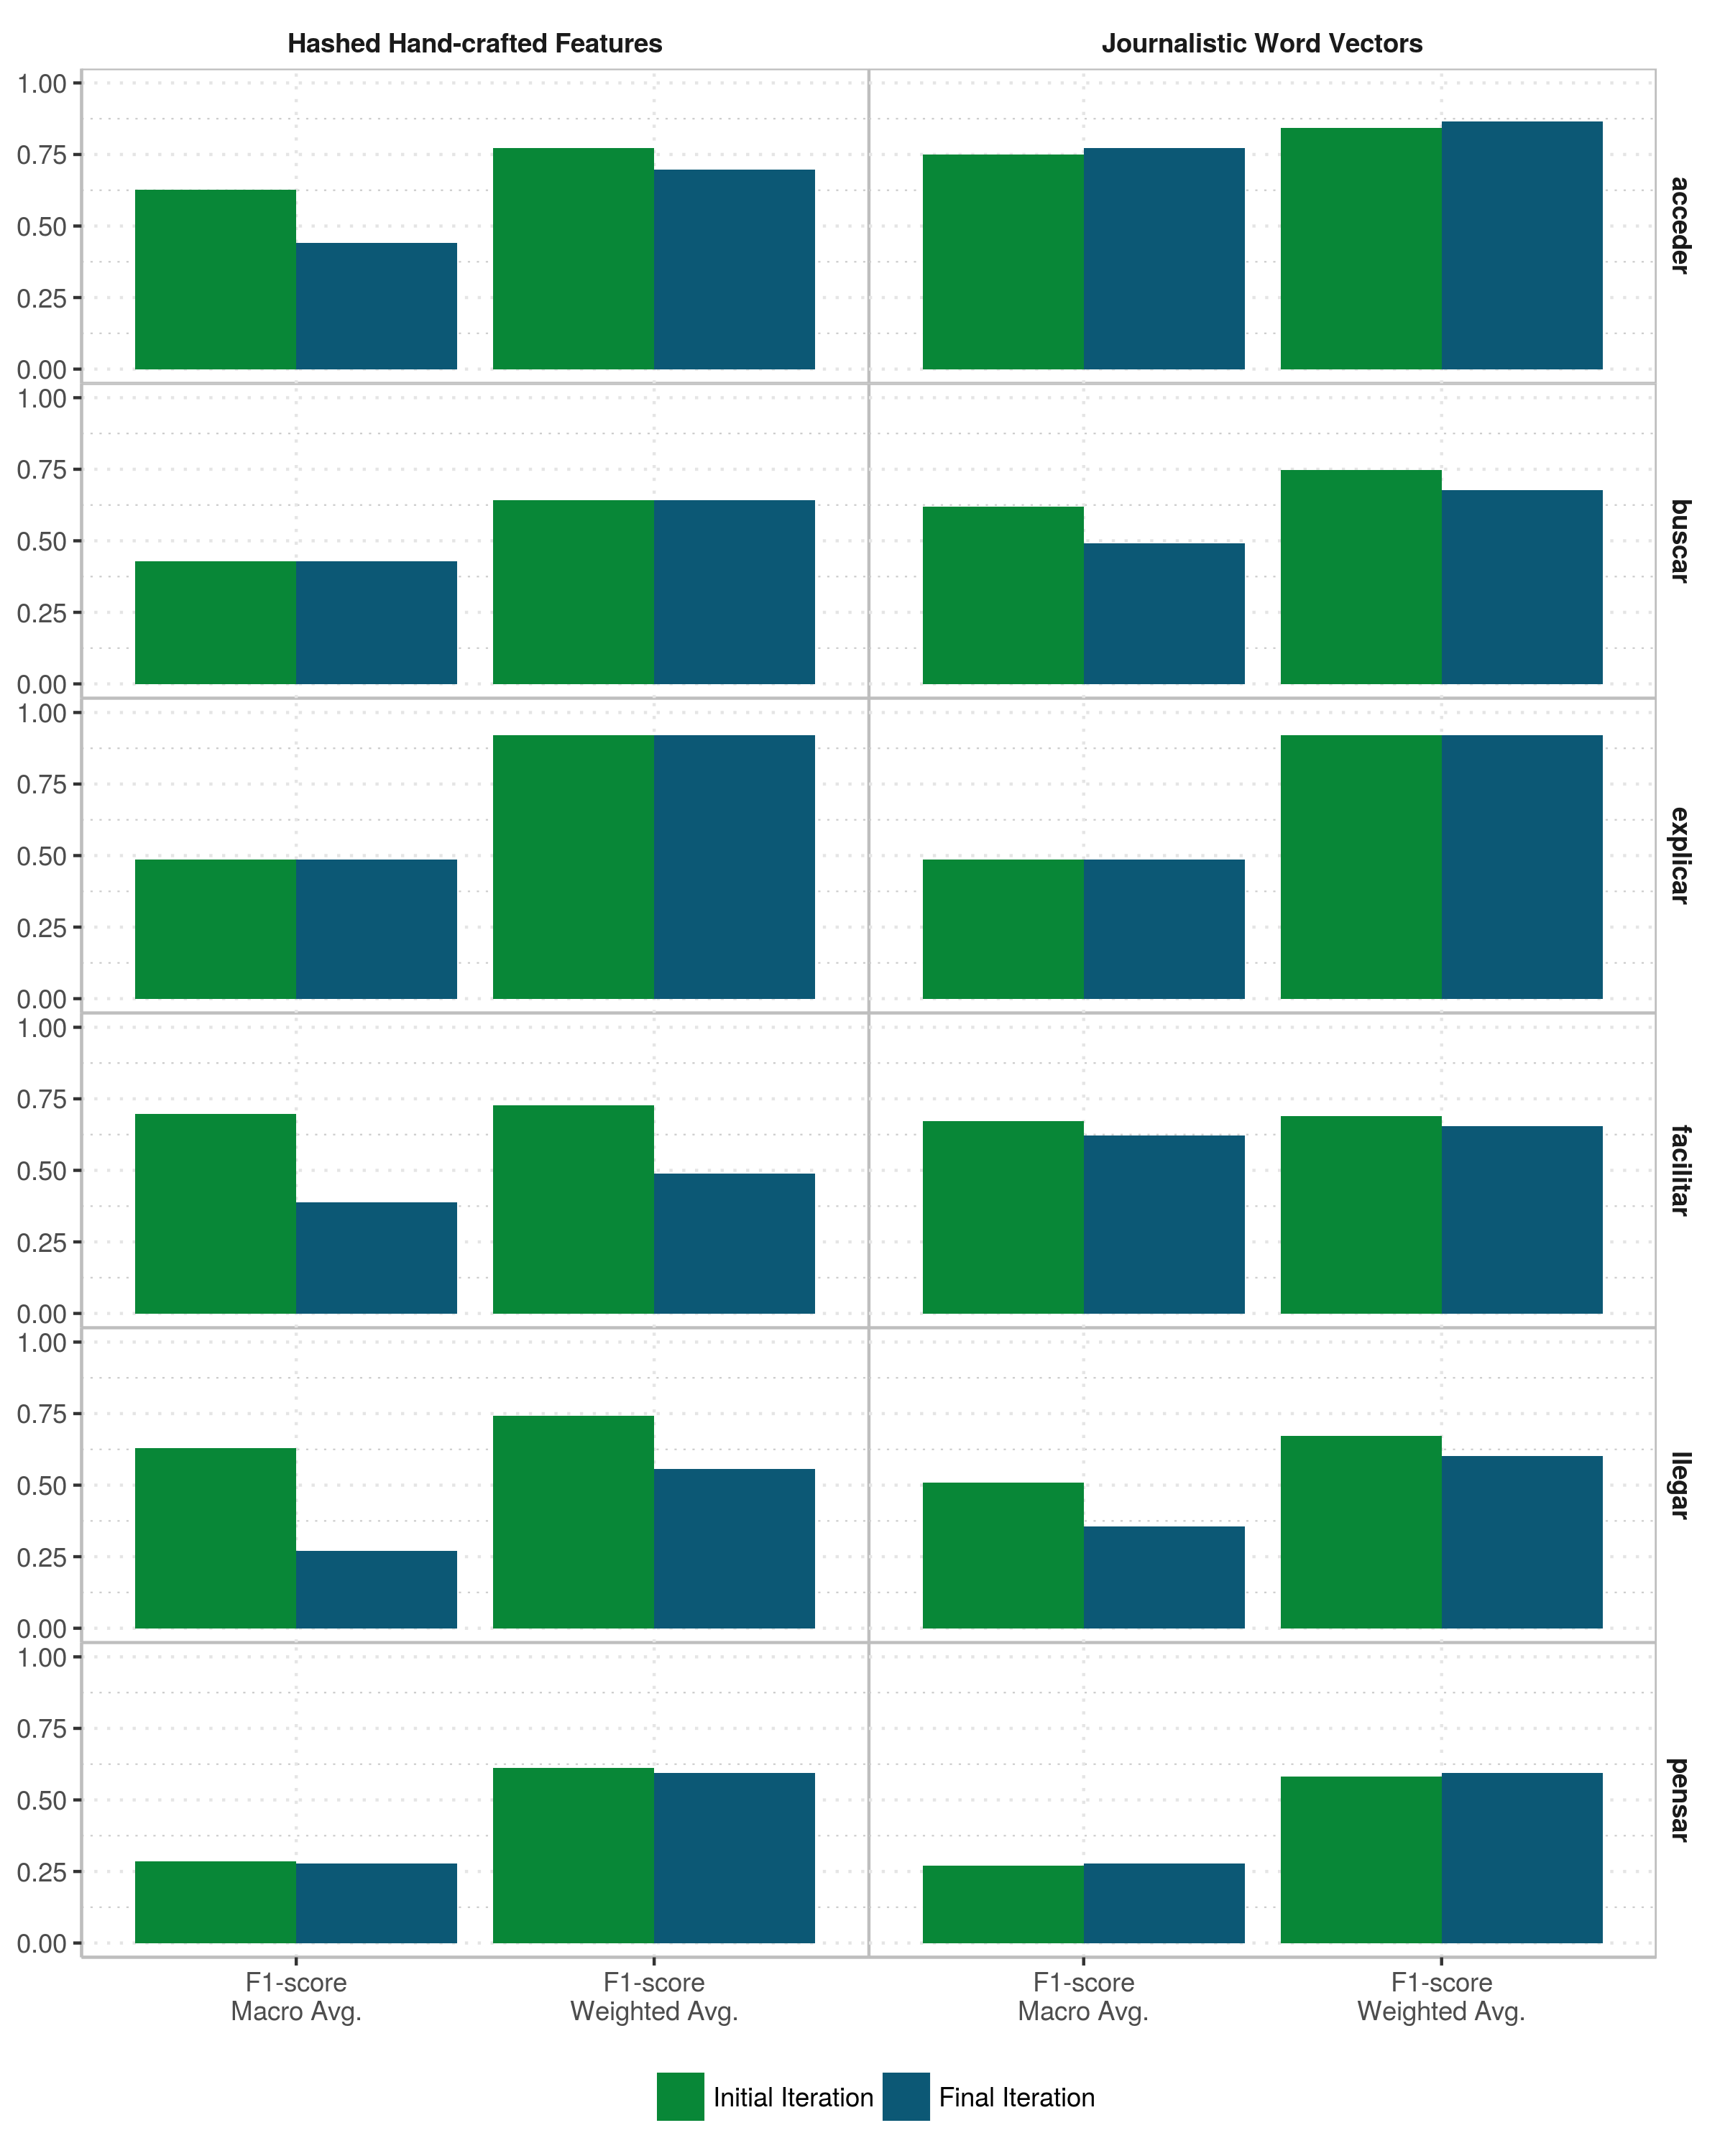
\includegraphics[height=.9\textheight,width=\textwidth,keepaspectratio]
    {plots/selflearning/test_results}
  \caption{Comparison of macro and weighted averaged F1-score before and after
  the self-learning algorithm's iterations}
  \label{fig:self-learning:test_performance}
\end{figure}

Figure \ref{fig:self-learning:test_performance} reports the performance results
on the test corpus before and after self-learning for each of the token lemmas
I presented in Section \ref{sec:self-learning:resources}. The plot is a bar
plot structured in the following way:

\begin{itemize}
  \item Each row shows the results for a token lemma: ``acceder'', ``buscar'',
    ``explicar'', ``facilitar'', ``llegar'', and ``pensar''.
  \item Each column stands for a feature representation: hand-crafted hashed
    features and journalistic word vectors.
  \item Each group of bars in each plot represents a metric: F1-score macro
    average and F1-score weighted average.
  \item Each bar plot in a different color inside a group represents the
    evaluation moment: initial iteration and final iteration.
  \item The bar plot represents the value of the metric.
\end{itemize}

As explained in Section \ref{sec:supervised:performance:metrics}, the weighted
average is useful to show the performance of the algorithm given the class
distribution (i.e. most frequent classes are more important in the final
result). On the other hand, the macro average is useful to see the performance
in less frequent classes. Then the spread between the macro and weighted
average shows how biased is the algorithm to the most frequent class.

Note that, as described in the previous chapter, word embeddings have worse
average performance than hand-crafted features. However, in two of the token
verbs shown here, word embeddings perform better than hand-crafted features, in
one of the verbs they perform at the same level and in three cases they perform
slightly worse. Actually, even if the average was different, the median was
very similar for word embeddings and hand-crafted features, so we can still
consider that these token verbs are representative of the population.

The figure shows that, except for two lemmas, hand-crafted features lose
performance after the self-learning algorithm ends. In none of the lemmas the
algorithm improves the performance over the original model without the new
data. For word embeddings the case is a little different, as in half of the
lemmas it does not lose performance, and it even improves in two of them. 

Comparing the loss in performance for the two different representations, the
drop is stronger for hand-crafted features, specially in the macro average.
From this results I can hypothesize that for hand-crafted features the
self-learning algorithm is more prone to add instances of the most frequent
class. This impacts in the performance of less frequent classes and is the
reason why the macro average drop in performance is much larger.

This drop in the performance measured by the macro average for word vectors is
not as pronounced as for hand-crafted features. Moreover, the general drop in
performance, in the cases when it happens, is not as big as for hand-crafted
features even if the latter have better performance for the initial iteration
(e.g. ``facilitar'', ``llegar'').

It can be concluded that, in general terms, word vectors work better than
hand-crafted features in this setting. This gives a strong indication of the
bias of the domain in the task. Hand-crafted features may have better
performance in the task with the original supervised dataset but they do not
generalize well to a bigger domain. In this case word embeddings provide a
better representation because, as we saw on the previous chapter, recalling
Hypothesis \ref{hyp:embeddings:2}, word embeddings have less tendency to
overfit a model. This is crucial in a setting like self-learning where new
examples are annotated automatically. In this setting, a better representation
makes the model adapt better to new data. I.e, hand-crafted features are
overfitting the model to the initial labeled dataset and that overfitting is
being transferred to the self-learning algorithm decisions regarding instances
to annotate automatically, producing a drift with a bias to the majority class.
Therefore, I can conclude that word vectors yield a better generalization of
the data for unseen examples.

The results do not show enough evidence to accept Hypothesis
\ref{hyp:self-learning:1}. In particular, hand-crafted features show evidence
to reject the Hypothesis as the general performance degrades after the
self-learning algorithm runs. Nevertheless, when word embeddings are integrated
in the setting, results are stronger to accept the Hypothesis, even if not
conclusive.

\subsection{Hypothesis \ref{hyp:self-learning:2}}\label{sec:self-learning:hyp:2}

The present section discusses the results I found regarding Hypothesis
\ref{hyp:self-learning:2}. The Hypothesis stated that the model trained after
each self-learning iteration, thus adding new data from unlabeled sources,
increased the average certainty to predict the class of new unseen examples.
Behind this hypothesis there is the assumption that the model, by adding new
unlabeled examples, can represent new examples better.

\begin{figure}[htb!]
  \centering
  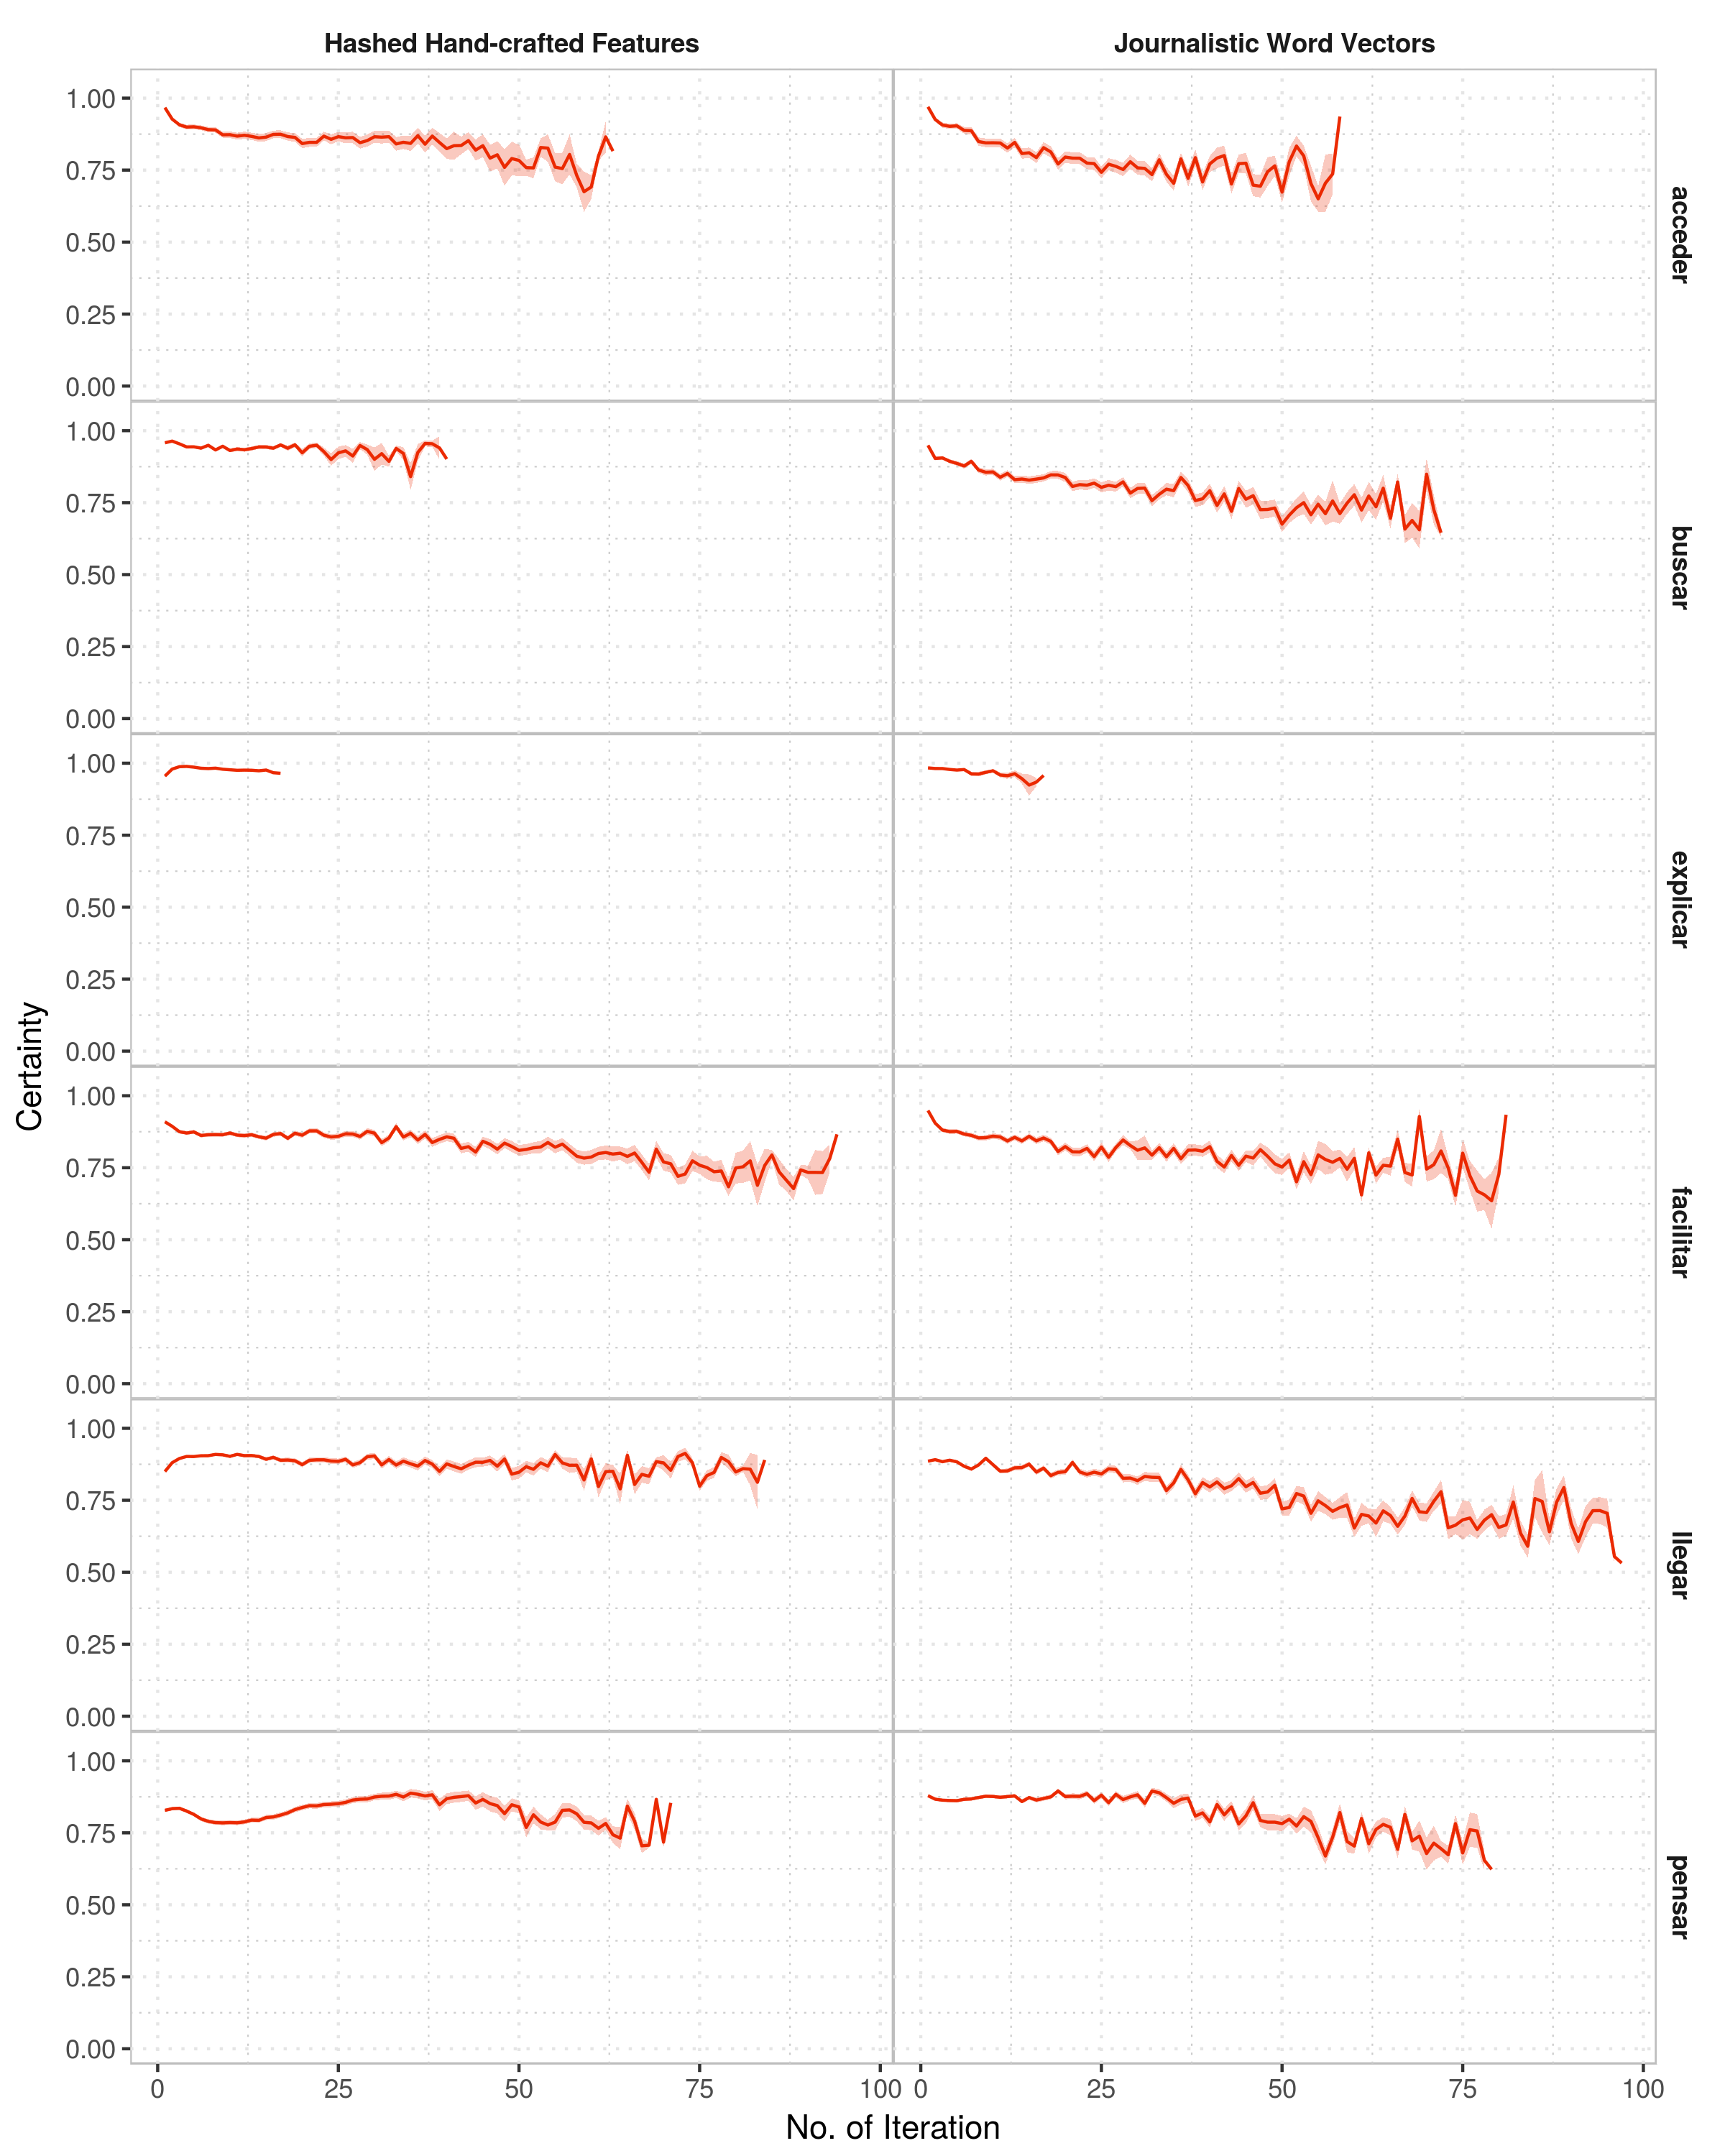
\includegraphics[height=.9\textheight,width=\textwidth,keepaspectratio]
    {plots/selflearning/certainty_progression}
  \caption{Average certainty to predict new classes for each self-learning
  iteration}
  \label{fig:self-learning:certainty}
\end{figure}

Figure \ref{fig:self-learning:certainty} shows the average certainty of the
model on new examples throughout the self-learning iterations. The data is
obtained running Experiment \ref{exp:self-learning:2}, which records the
predicted classes' certainty of the model for all the new examples from the
pool of unlabeled data. The metric to measure this is an unweighted average
described in Metric \ref{met:5}. The figure shows a line plot with the
following structure:

\begin{itemize}
  \item Each row shows the results for a token lemma: ``acceder'', ``buscar'',
    ``explicar'', ``facilitar'', ``llegar'', and ``pensar''.
  \item Each column stands for a feature representation: hand-crafted hashed
    features and journalistic word vectors.
  \item The x-coordinate axis represents the iteration number in the
    self-learning algorithm.
  \item The y-coordinate axis represents the raw count of features.
  \item The solid darker line represents the mean of certainty the mode has
    over the unlabeled data it is predicting.
  \item The shadowed area, which has a lighter color, represents the standard
    error of the mean of the certainty.
\end{itemize}

The plots I show are quite complex to follow and reason about. What is most
noticeable is that the certainty of the algorithm over the unseen examples is
less uniform as more iterations are added. In contrast to what I originally
assumed in Hypothesis \ref{hyp:self-learning:2}, the algorithm shows a lower
certainty over new examples. 

It is noticeable that hand-crafted features start with a certainty that is more
uniform through the initial iterations. Nonetheless as iterations go further,
certainty becomes more and more variable. Meanwhile, word vectors always show a
variable certainty over unseen examples. How certainty evolves through the
iterations in the self-learning algorithm gives us the idea that the model is
not converging, at least not in terms measured by certainty.

It is clear that the new examples add more uncertainty to the model, something
that becomes worse by adding more examples. Since the algorithm is drifting to
classify examples into the most frequent class, one would expect that the
certainty for the majority class is increased. However, what actually happens
is that the majority class accumulates many different examples. Most of these
examples are poorly characterized by the model, because most of their features
are unknown to the model. Thus, the classifier does not have a big certainty
over the majority class. Instead, it seems that many instances are classified
in that class only because the model does not have enough information to
classify them in any class, and it simply chooses the most probable one. In
sum, integrating more examples does not seem to increase the certainty because
they are not integrated in a smart manner, but relying only on the probability
of the majority class. Then, no new examples are added to minority classes (and
their certainty does not increase), and examples added to the majority class
only contribute to disperse the certainty.

\subsection{Hypothesis \ref{hyp:self-learning:3}}\label{sec:self-learning:hyp:3}

Hypothesis \ref{hyp:self-learning:3} is based on what I discussed in previous
chapters regarding the tendency of a model to overfit the training data. It
states that adding new unseen examples automatically through the self-learning
algorithm helps reducing the overfit of the model.

The Hypothesis is tested with the results reported by Experiment
\ref{exp:self-learning:3}. The experiment is similar to what I did in the
previous chapter to see the evolution of the {\em error due to variance} using
the learning curve of the model. The main difference lies in that in previous
chapters I needed to split the labeled dataset in order to simulate adding new
examples to a model. Thus, in previous chapters, new added examples were
actually labeled examples I left outside in the beginning.

Self-learning gives me the possibility to explore how real unseen examples
affect the tendency to overfit of a model measured by the learning curve
defined as Metric \ref{met:3} in Chapter \ref{chapter:supervised}.

There are however two possible views of the learning curve in this case. The
first approach is by plotting the curve in function of the iterations of the
algorithm. The second approach is to plot the curve in function of the number
of examples used for training.

The first approach is more focused on how the self-learning algorithm works
rather on how the model evolves. In each iteration the number of examples added
can be high or low. As I did not limit the number of new examples to add, there
is no certain way of telling how many the algorithm is adding for each
iteration. What the results show in this case is rather how the added examples
affect the model in that iteration. The second approach is more analogous to
what is shown in previous chapters, as the plot is done based on the number of
examples of the training dataset rather than the iteration they were added.

Both views are useful on their own ways, nevertheless for comparison with the
previous methods I opted for analyzing the second approach as it is closer to
what I already discussed for supervised and word embeddings approaches before.

\begin{figure}[htb!]
  \centering
  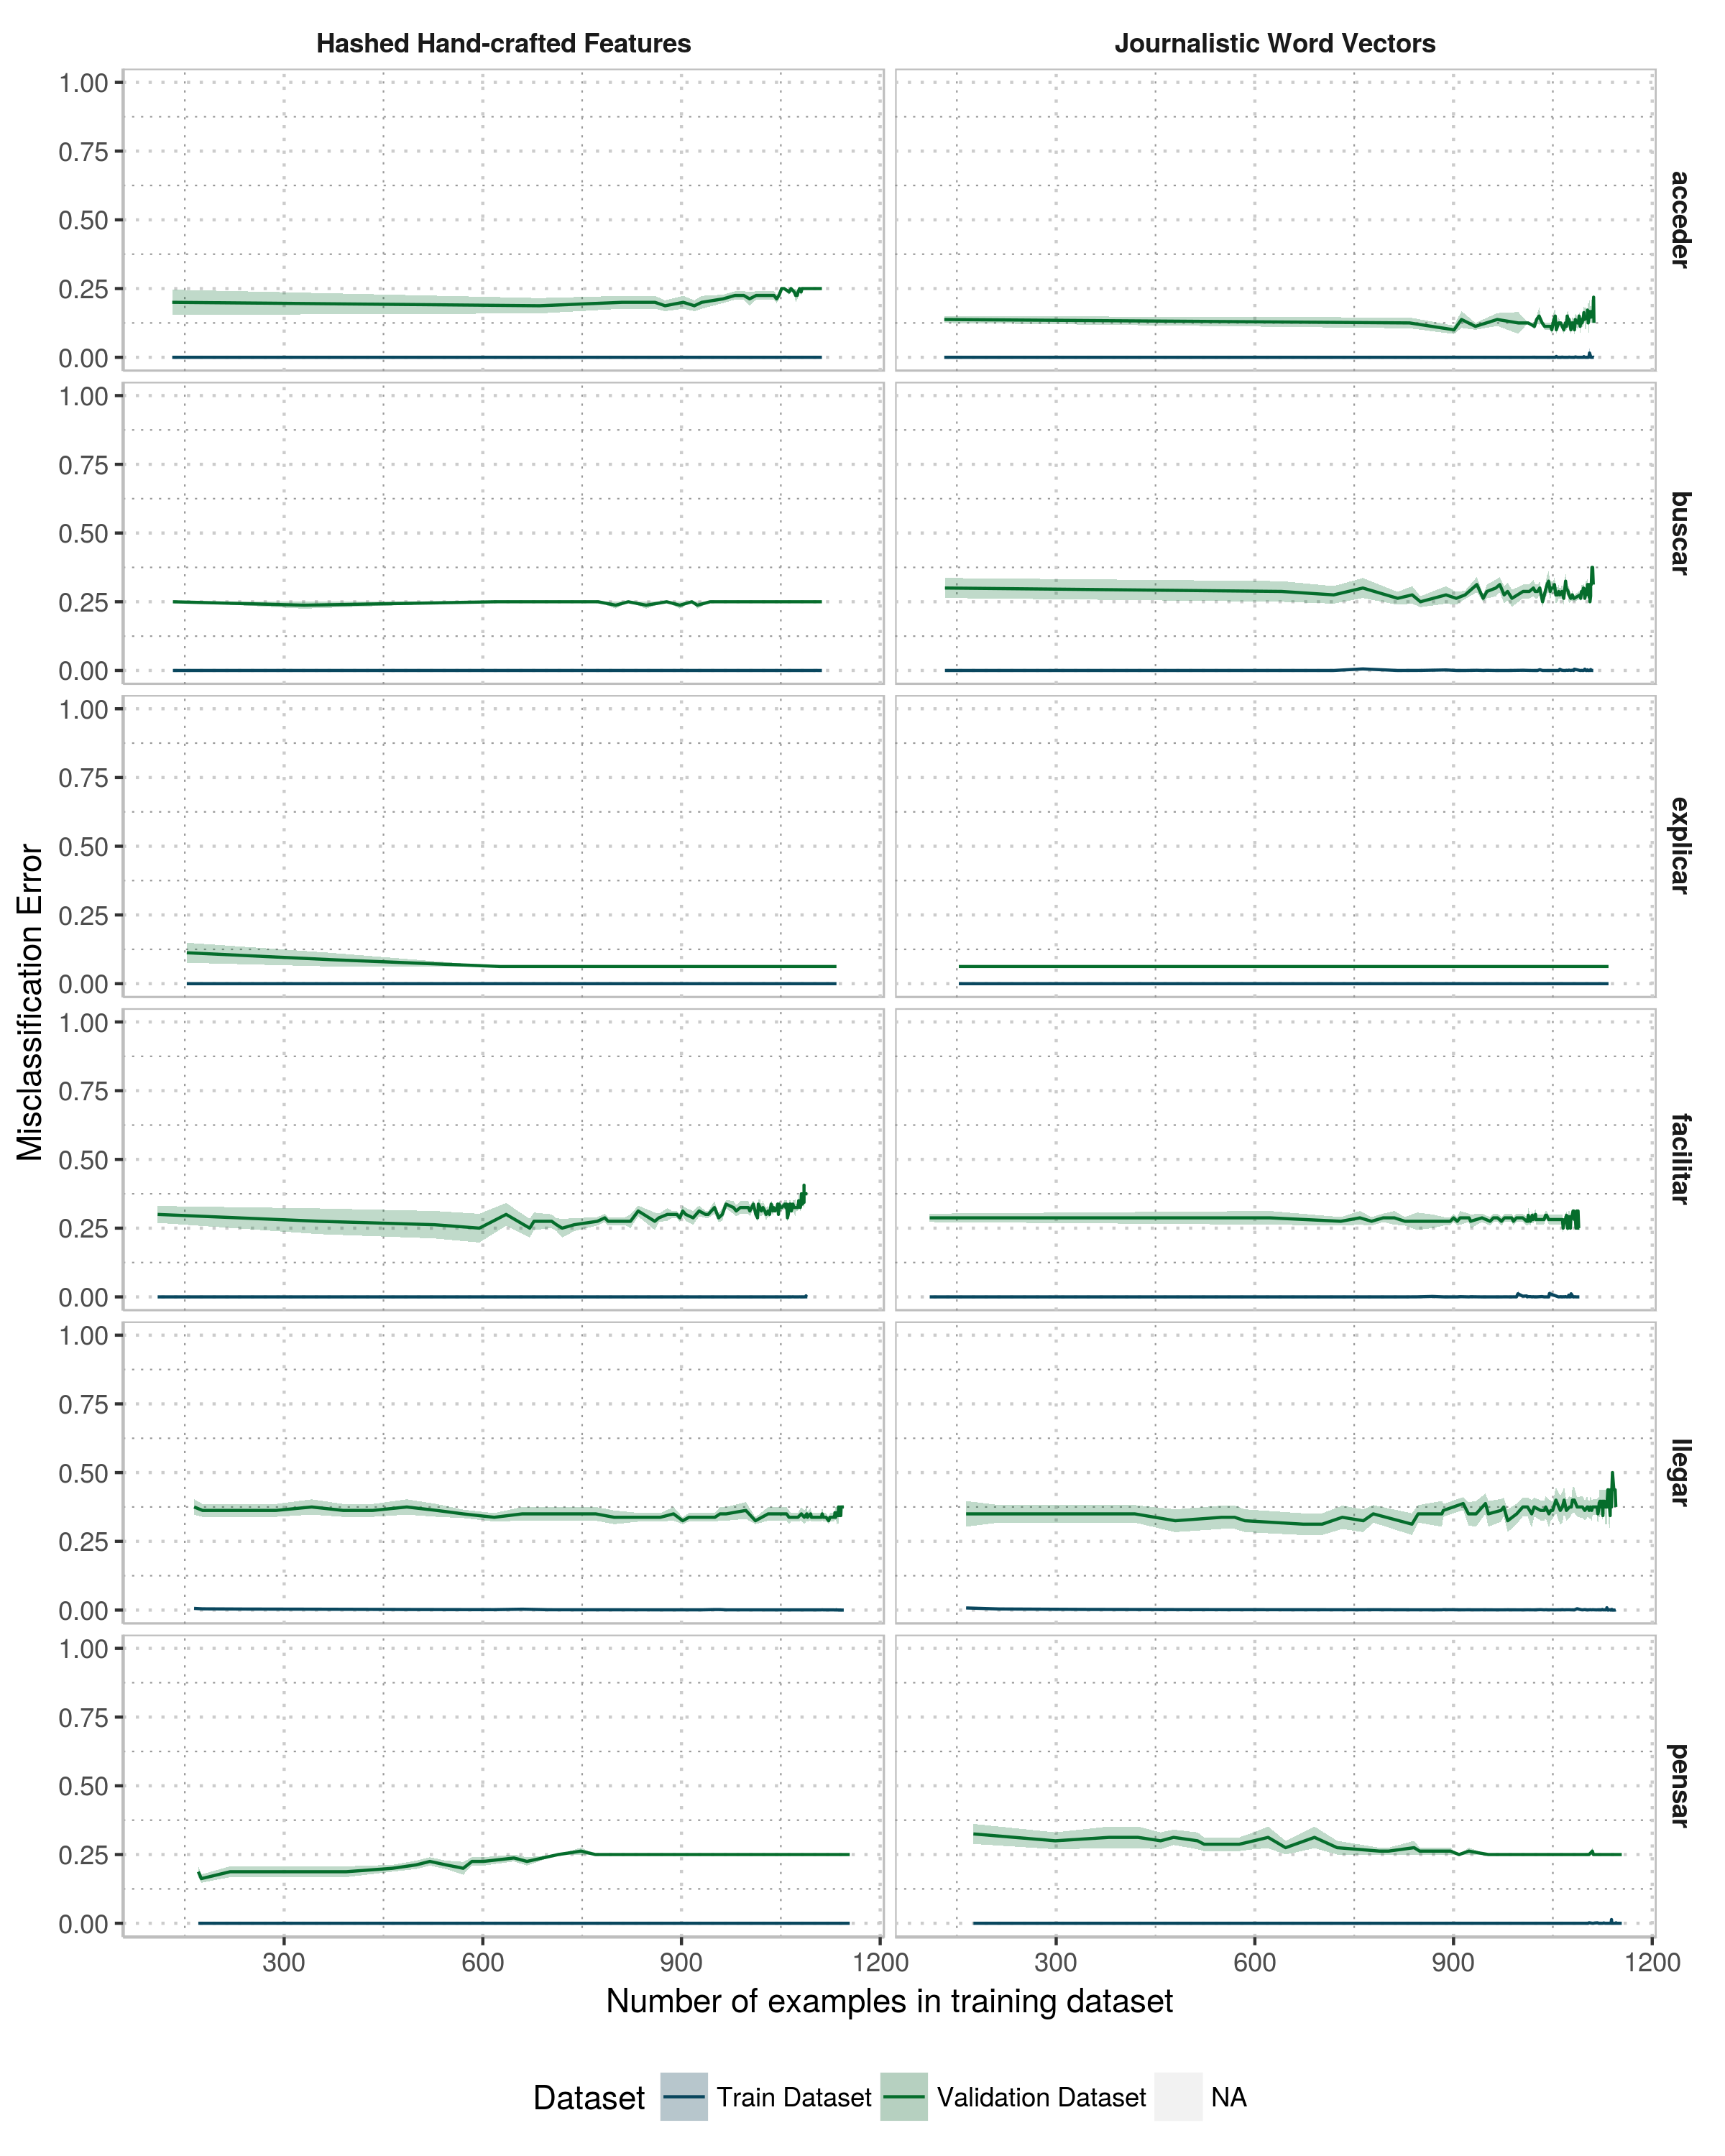
\includegraphics[height=.9\textheight,width=\textwidth,keepaspectratio]
    {plots/selflearning/overfit_measure_per_examples}
  \caption{Learning curve as a function of the number of examples added by the
  self-learning algorithm}
  \label{fig:self-learning:overfit}
\end{figure}

Figure \ref{fig:self-learning:overfit} shows the learning curve plot as a
function of the number of examples of the training dataset. The structure of
the learning curve plot is as follows:

\begin{itemize}
  \item Each row shows the results for a token lemma: ``acceder'', ``buscar'',
    ``explicar'', ``facilitar'', ``llegar'', and ``pensar''.
  \item Each column stands for a feature representation: hand-crafted hashed
    features and journalistic word vectors.
  \item The x-coordinate axis represents the number of examples in the
    self-learning algorithm.
  \item There are two colors representing the datasets: train and validation
    (in this case is the validation set).
  \item The solid darker lines represent the mean of misclassification error
    trough the different iterations of the datasets over all the models.
  \item The shadowed area, which have a lighter color, represent the standard
    error of the mean of the misclassification error.
\end{itemize}

Recall I am limiting my unlabeled pool of data to 1000 unannotated examples and
that is why none of the plots go beyond 1150 examples total (that is the
original supervised dataset plus the automatically annotated examples).

A first look into the graphics shows that the misclassification error drops a
little after the first set of automatically annotated examples is added. This
is more or less uniform for all the lemmas for the first increments. If I take
into consideration that these examples are added in the first iterations, it is
interesting to see that the first iterations are the ones adding up to improve
the generalization of the model. This happens regardless of the representation
used.

It is also interesting to see that in general terms the shadowed area, which is
the standard error of the mean for the misclassification error, becomes
narrower the more examples are added. This means the model has less variance
over the validation dataset. This is an indication of the model reducing the
error due to variance, which is one of our indicators of reduced overfitting.

Besides that, it is striking how the error in the validation dataset starts to
become highly irregular for every new example added. This happens in most of
the cases for the examples added in later iterations. This can be due to the
fact that in the final iterations of the algorithm, the tolerated error level
in the validation dataset is bigger. Indeed, the tolerated error in the
validation dataset is slowly increased by the method as iterations go, and
until it reaches the stopping threshold. This is specially relevant for the
case of word embeddings. It may require a further analysis left for future work
for now.

This tendency could be further explore and systematized to the point that it
can be used as a stopping criterion for the algorithm. Indeed, the difference
in validation and training error over the iterations could be a good stopping
criterion.

\subsection{Hypothesis \ref{hyp:self-learning:4}}\label{sec:self-learning:hyp:4}

Hypothesis \ref{hyp:self-learning:4} is based on what I talked about previously
regarding model coverage. To measure the coverage I do so by counting the
features the model recognizes. For hand-crafted features this means all the
features obtained from the training data (which includes words, tokens,
part-of-speech, etc. as explained in Section \ref{sec:supervised:features}).
For the case of word embeddings, the features are the words surrounding the
verb to disambiguate and the position relative to that verb. There is more than
one way to measure the coverage of a model by its features. Hypothesis
\ref{hyp:self-learning:4} is interested in showing that the model increases
it is number of features by adding new examples so I get the raw count of the
total number of features the model has in the training dataset over the
self-learning iterations.

\begin{figure}[htb!]
  \centering
  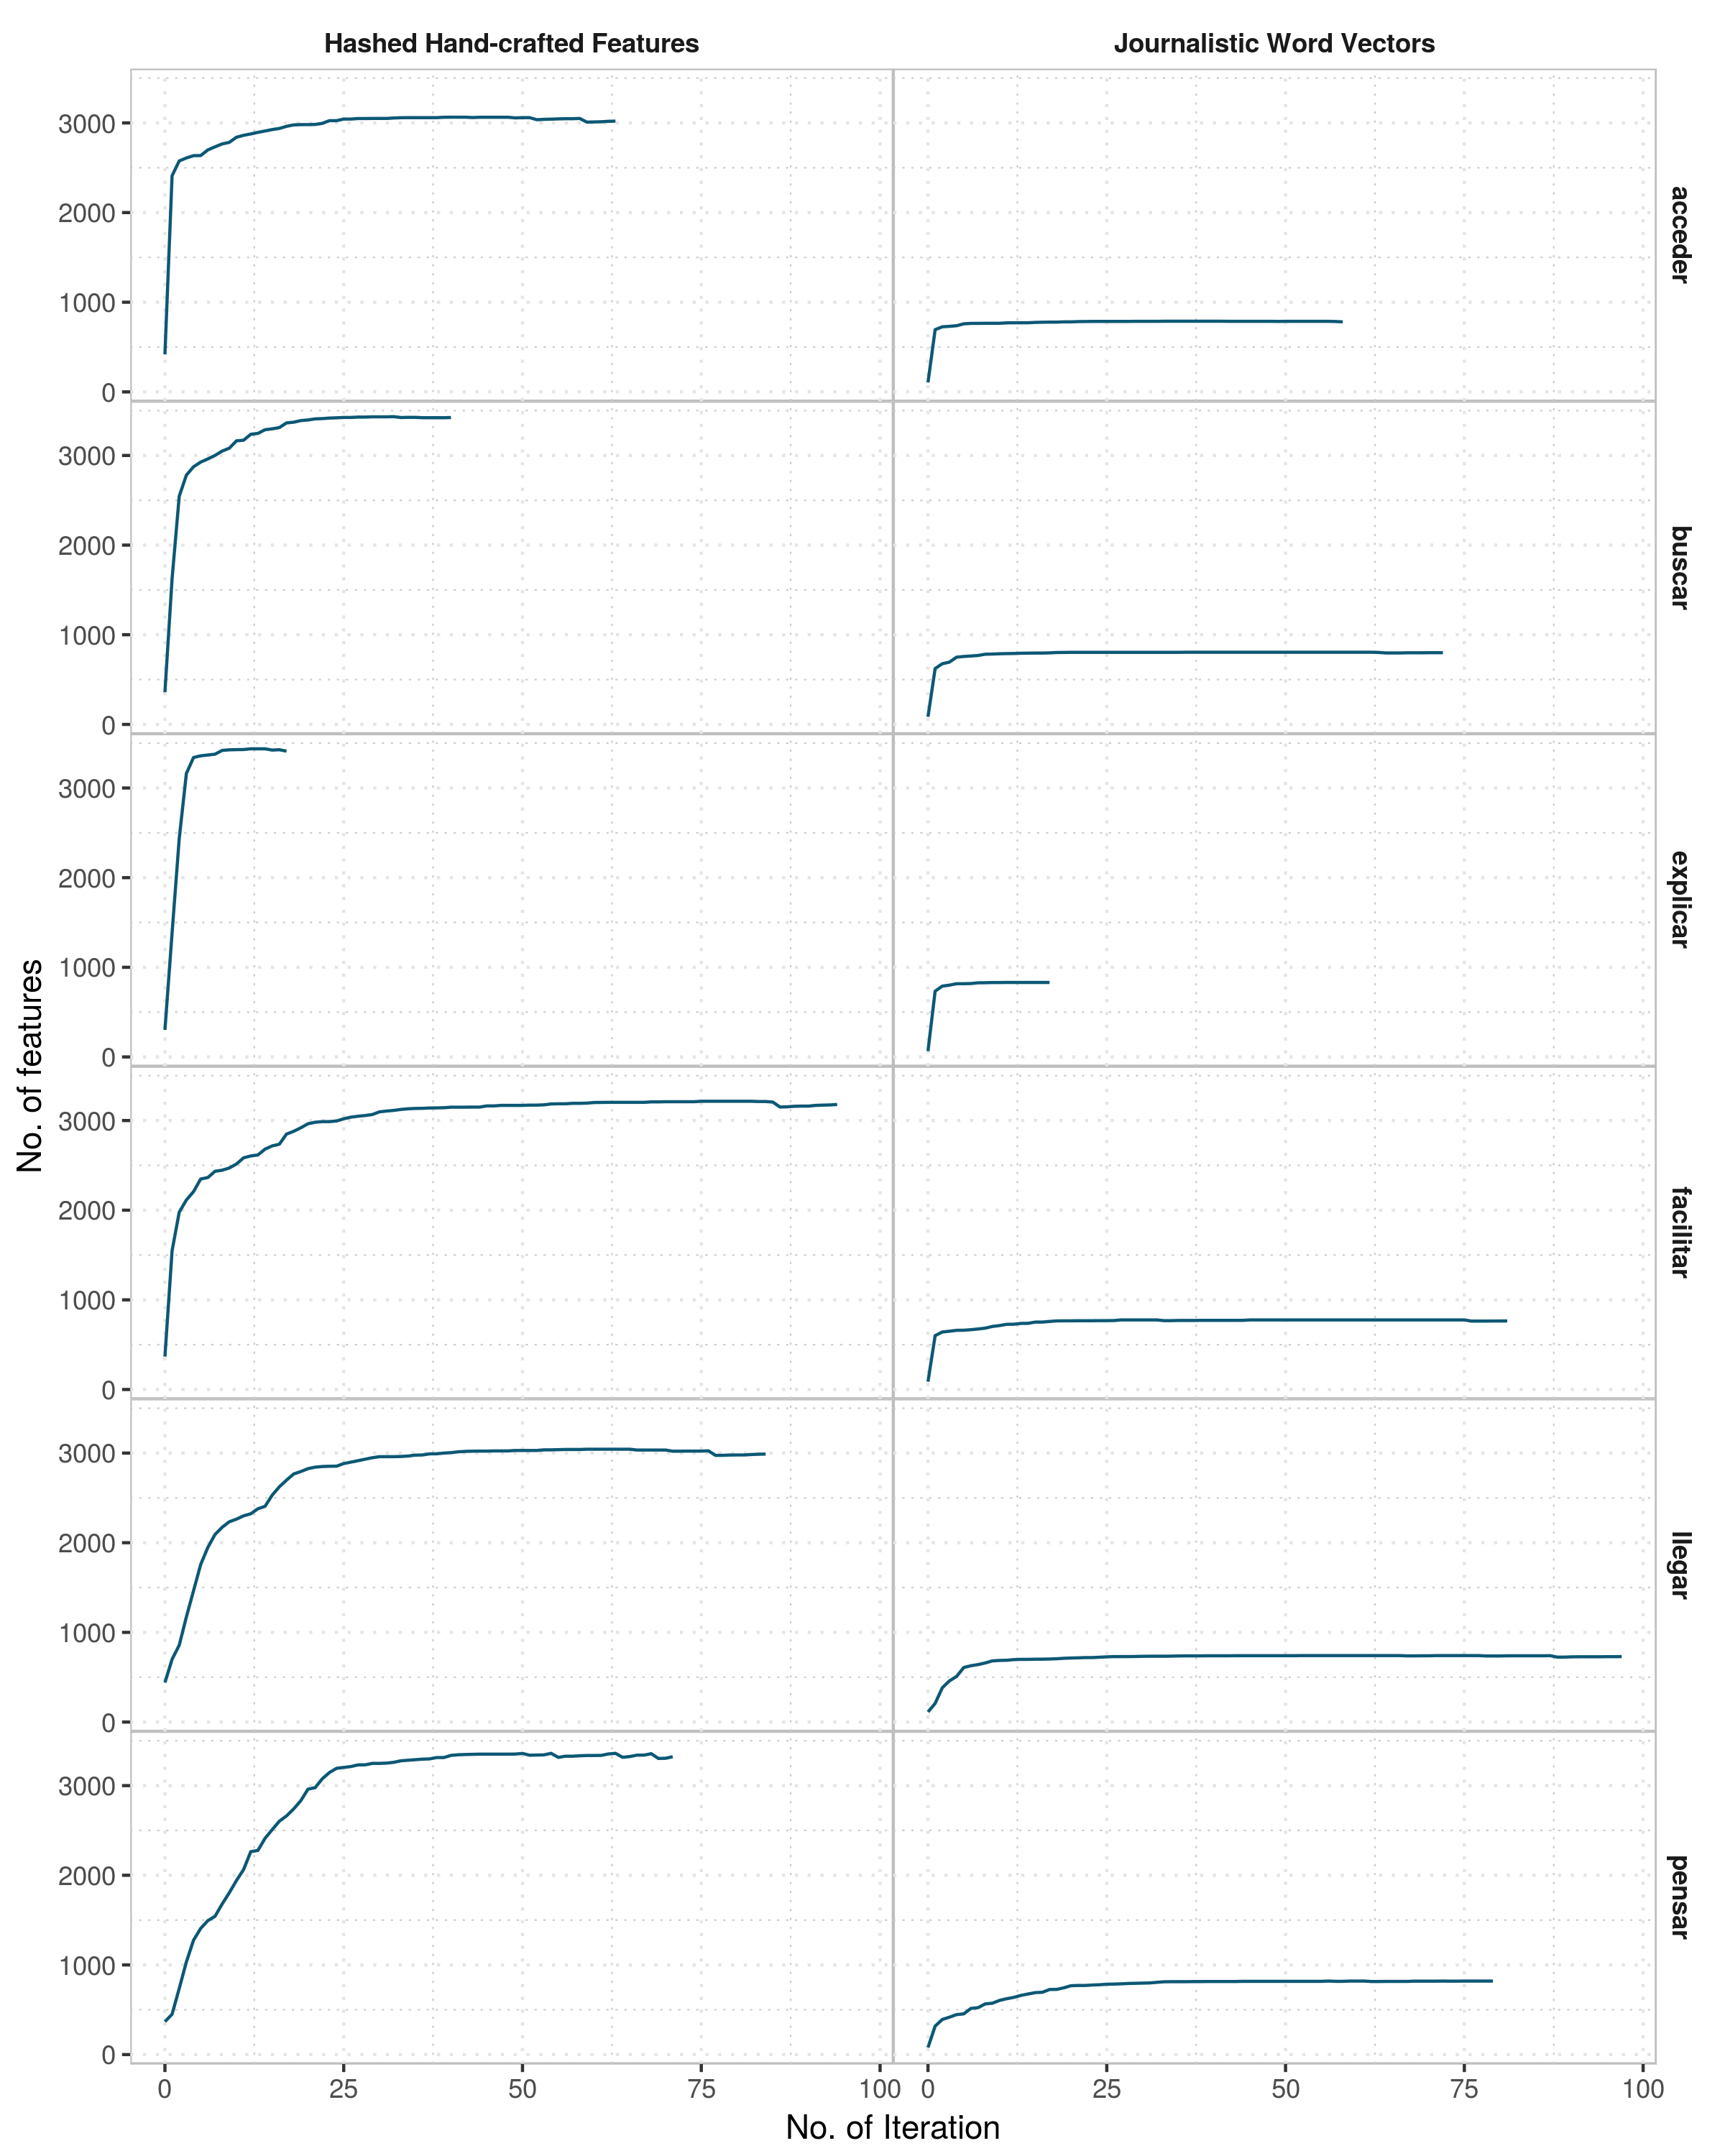
\includegraphics[height=.9\textheight,width=\textwidth,keepaspectratio]
    {plots/selflearning/features_growth_total}
  \caption{Features' growth in the model across self-learning iterations}
  \label{fig:self-learning:features_growth_total}
\end{figure}

Figure \ref{fig:self-learning:features_growth_total} reports the features'
growth of the model across the self-learning iterations. That is the total
number of unique features up to that iteration obtained both from the original
supervised dataset and the automatically annotated data. The figure shows a
line plot with the following structure:

\begin{itemize}
  \item Each row shows the results for a token lemma: ``acceder'', ``buscar'',
    ``explicar'', ``facilitar'', ``llegar'', and ``pensar''.
  \item Each column stands for a feature representation: hand-crafted hashed
    features and journalistic word vectors.
  \item The x-coordinate axis represents the iteration number in the
    self-learning algorithm.
  \item The y-coordinate axis represents the raw count of unique features.
\end{itemize}

From the figure it is visually striking that most of the new features are
acquired in the first iterations of the self-learning algorithm. After that the
number of features stales. This is an indication of the algorithm adding lot of
examples in the first iterations while almost none in the following ones.

It is interesting to note the difference between hand-crafted features and word
vectors. It is natural because of what I explained previously regarding what is
that I am considering as features for each type of representation. The pool of
features for the word embeddings model is much smaller than for hand-crafted
features. Regardless of the scale, there is a shared pattern for both
representations regarding the way the features in the models grow.

These results show that the model effectively increases the features associated
to it, which is stated by Hypothesis \ref{hyp:self-learning:4}. The hypothesis
is accepted in that way. However, this is not necessarily an increase in the
coverage of the model as I will show in further sections.

\subsection{Hypothesis \ref{hyp:self-learning:5}}\label{sec:self-learning:hyp:5}

In this section I discuss the results regarding Hypothesis
\ref{hyp:self-learning:5}. This hypothesis together with the following two in
this chapter are expected to be false (in contrast to the previous ones).
Hypothesis \ref{hyp:self-learning:5} states that self-learning helps improving
the performance of the model on each class uniformly.

To test this hypothesis I work on the results of Experiment
\ref{exp:self-learning:1} again. Remember that in that experiment the idea is
to evaluate the model over the held-out test dataset before and after running
the self-learning iterations. However, this time, instead of reporting the
averages defined in Metric \ref{met:1}, I show the F1-score for the most
frequent, second most frequent and, in some cases, third most frequent class of
the lemma. I do this because these are the classes of the token lemmas that
were not filtered out in the preprocessing of the corpus. From the 6 token
lemmas, 4 of them have only two senses with instances in the labeled dataset
(``acceder'', ``buscar'', ``explicar'', and ``facilitar''), and only 2 of them
have 3 senses with instances in the dataset (``llegar'' and ``pensar'').

\begin{figure}[htb!]
  \centering
  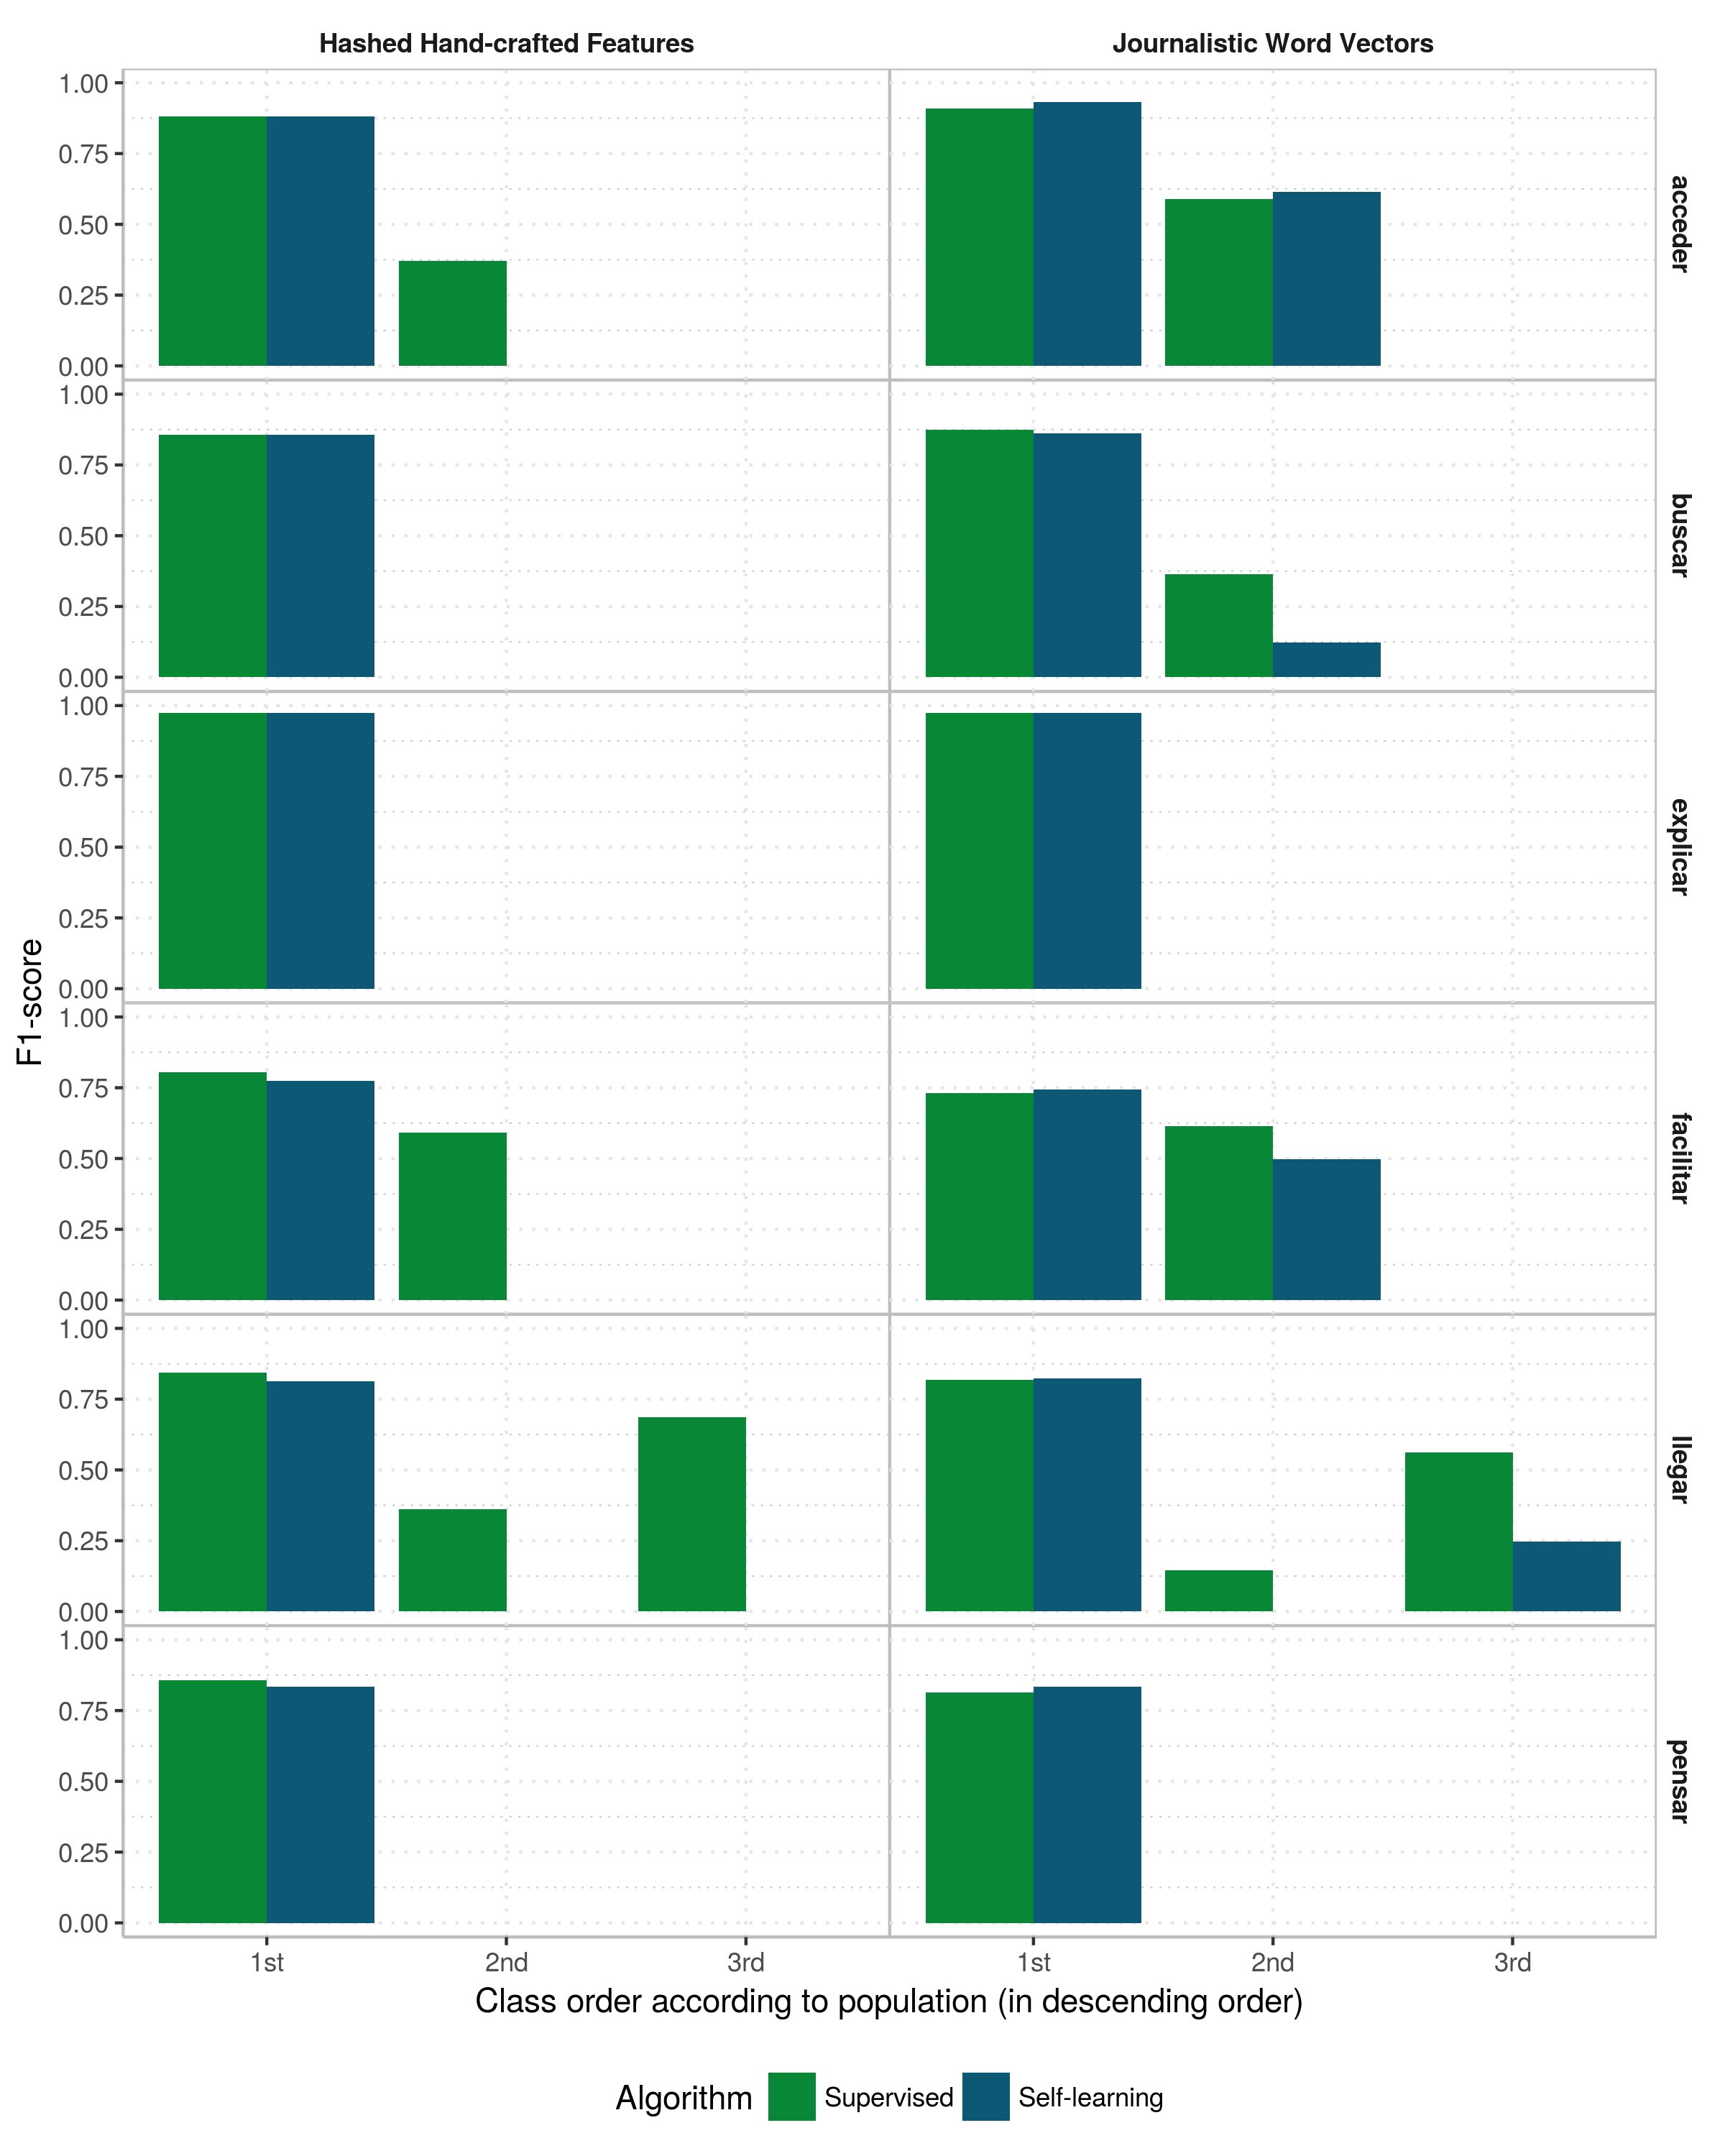
\includegraphics[height=.9\textheight,width=\textwidth,keepaspectratio]
    {plots/selflearning/per_sense_fscore}
  \caption{Comparison of F1-score for each class before and after the
  self-learning algorithm's iterations for the token lemmas}
  \label{fig:self-learning:per_class_performance}
\end{figure}

Figure \ref{fig:self-learning:per_class_performance} reports the performance
results on the test corpus for supervised (i.e. before the self-learning
iteration starts) and self-learning algorithms for each class (i.e. sense) of
each of the token lemmas I presented in Section
\ref{sec:self-learning:resources}. The plot is a bar plot structured in the
following way:

\begin{itemize}
  \item Each row shows the results for a token lemma: ``acceder'', ``buscar'',
    ``explicar'', ``facilitar'', ``llegar'', and ``pensar''.
  \item Each column stands for a feature representation: hand-crafted hashed
    features and journalistic word vectors.
  \item Each group of bars in each plot represents the class (i.e. sense) for
    that lemma. These are ordered according to number of occurrences of the
    class in the dataset.
  \item Each bar plot in a different color inside a group represents the
    algorithm: supervised (i.e. evaluation moment of the initial iteration),
    self-learning (i.e. evaluation moment of the final iteration after
    self-learning finishes).
  \item The height of the bar represents the value of the F1-score per each
    class.
\end{itemize}

Recall again that only the last two rows of the graphics have lemmas with 3
senses (i.e. ``llegar'' and ``pensar''). The first four lemmas can at most show
results for two senses.

From the figure it is clear that the self-learning algorithm is affecting
negatively the performance of all the classes that are not the most frequent
class. The only lemma in which there is a slight improvement in performance for
a class that is not the most frequent one is the lemma ``acceder'' and only
does so with the word embeddings representation.

This plot gives more information based on each class rather than obscuring
everything into an averaged metric. From it I can see that even though word
embeddings may have less performance in classes other than the most frequent,
the self-learning algorithm does not affect it as much as it does for
hand-crafted features. With hand-crafted features the F1-score directly drops
to zero for all classes other than the most frequent one. This is clearly a
sign of divergence to the most frequent class when new examples are added by
the self-learning algorithm.

The results are clear in this case and it is safe to reject Hypothesis
\ref{hyp:self-learning:5} as I originally thought.

\subsection{Hypothesis \ref{hyp:self-learning:6}}\label{sec:self-learning:hyp:6}

The next Hypothesis to test is \ref{hyp:self-learning:6}. This is an extension
of the explanation for the previous hypothesis as it states that the
representativity of each class in the dataset is maintained through all the
iterations of the self-learning algorithm. By representativity I mean the
number of classes as a proportion of the whole training dataset. This
Hypothesis is expected to be false and is a result of the self-learning
algorithm tendency to classify every new instance as the most frequent class.

Experiment \ref{exp:self-learning:5} is used in this section to report the
results of the self-learning algorithm with respect to the representativity of
each class through iterations. The experiment records the distribution of the
classes in the training dataset in each iteration. The metric to measure this
is the proportional count of occurrences each class, with respect to the whole
data available

To visualize these results I focus on two aspects I find relevant when
considering the hypothesis. First is the proportional count of number of
instances per class along the iterations of the algorithm. Second I want to
show how many examples of each class are added in each of the iterations of the
algorithm as a proportion of all the examples added in that iteration.

\subsubsection{Classes' population distribution across iterations}

\begin{figure}[htb!]
  \centering
  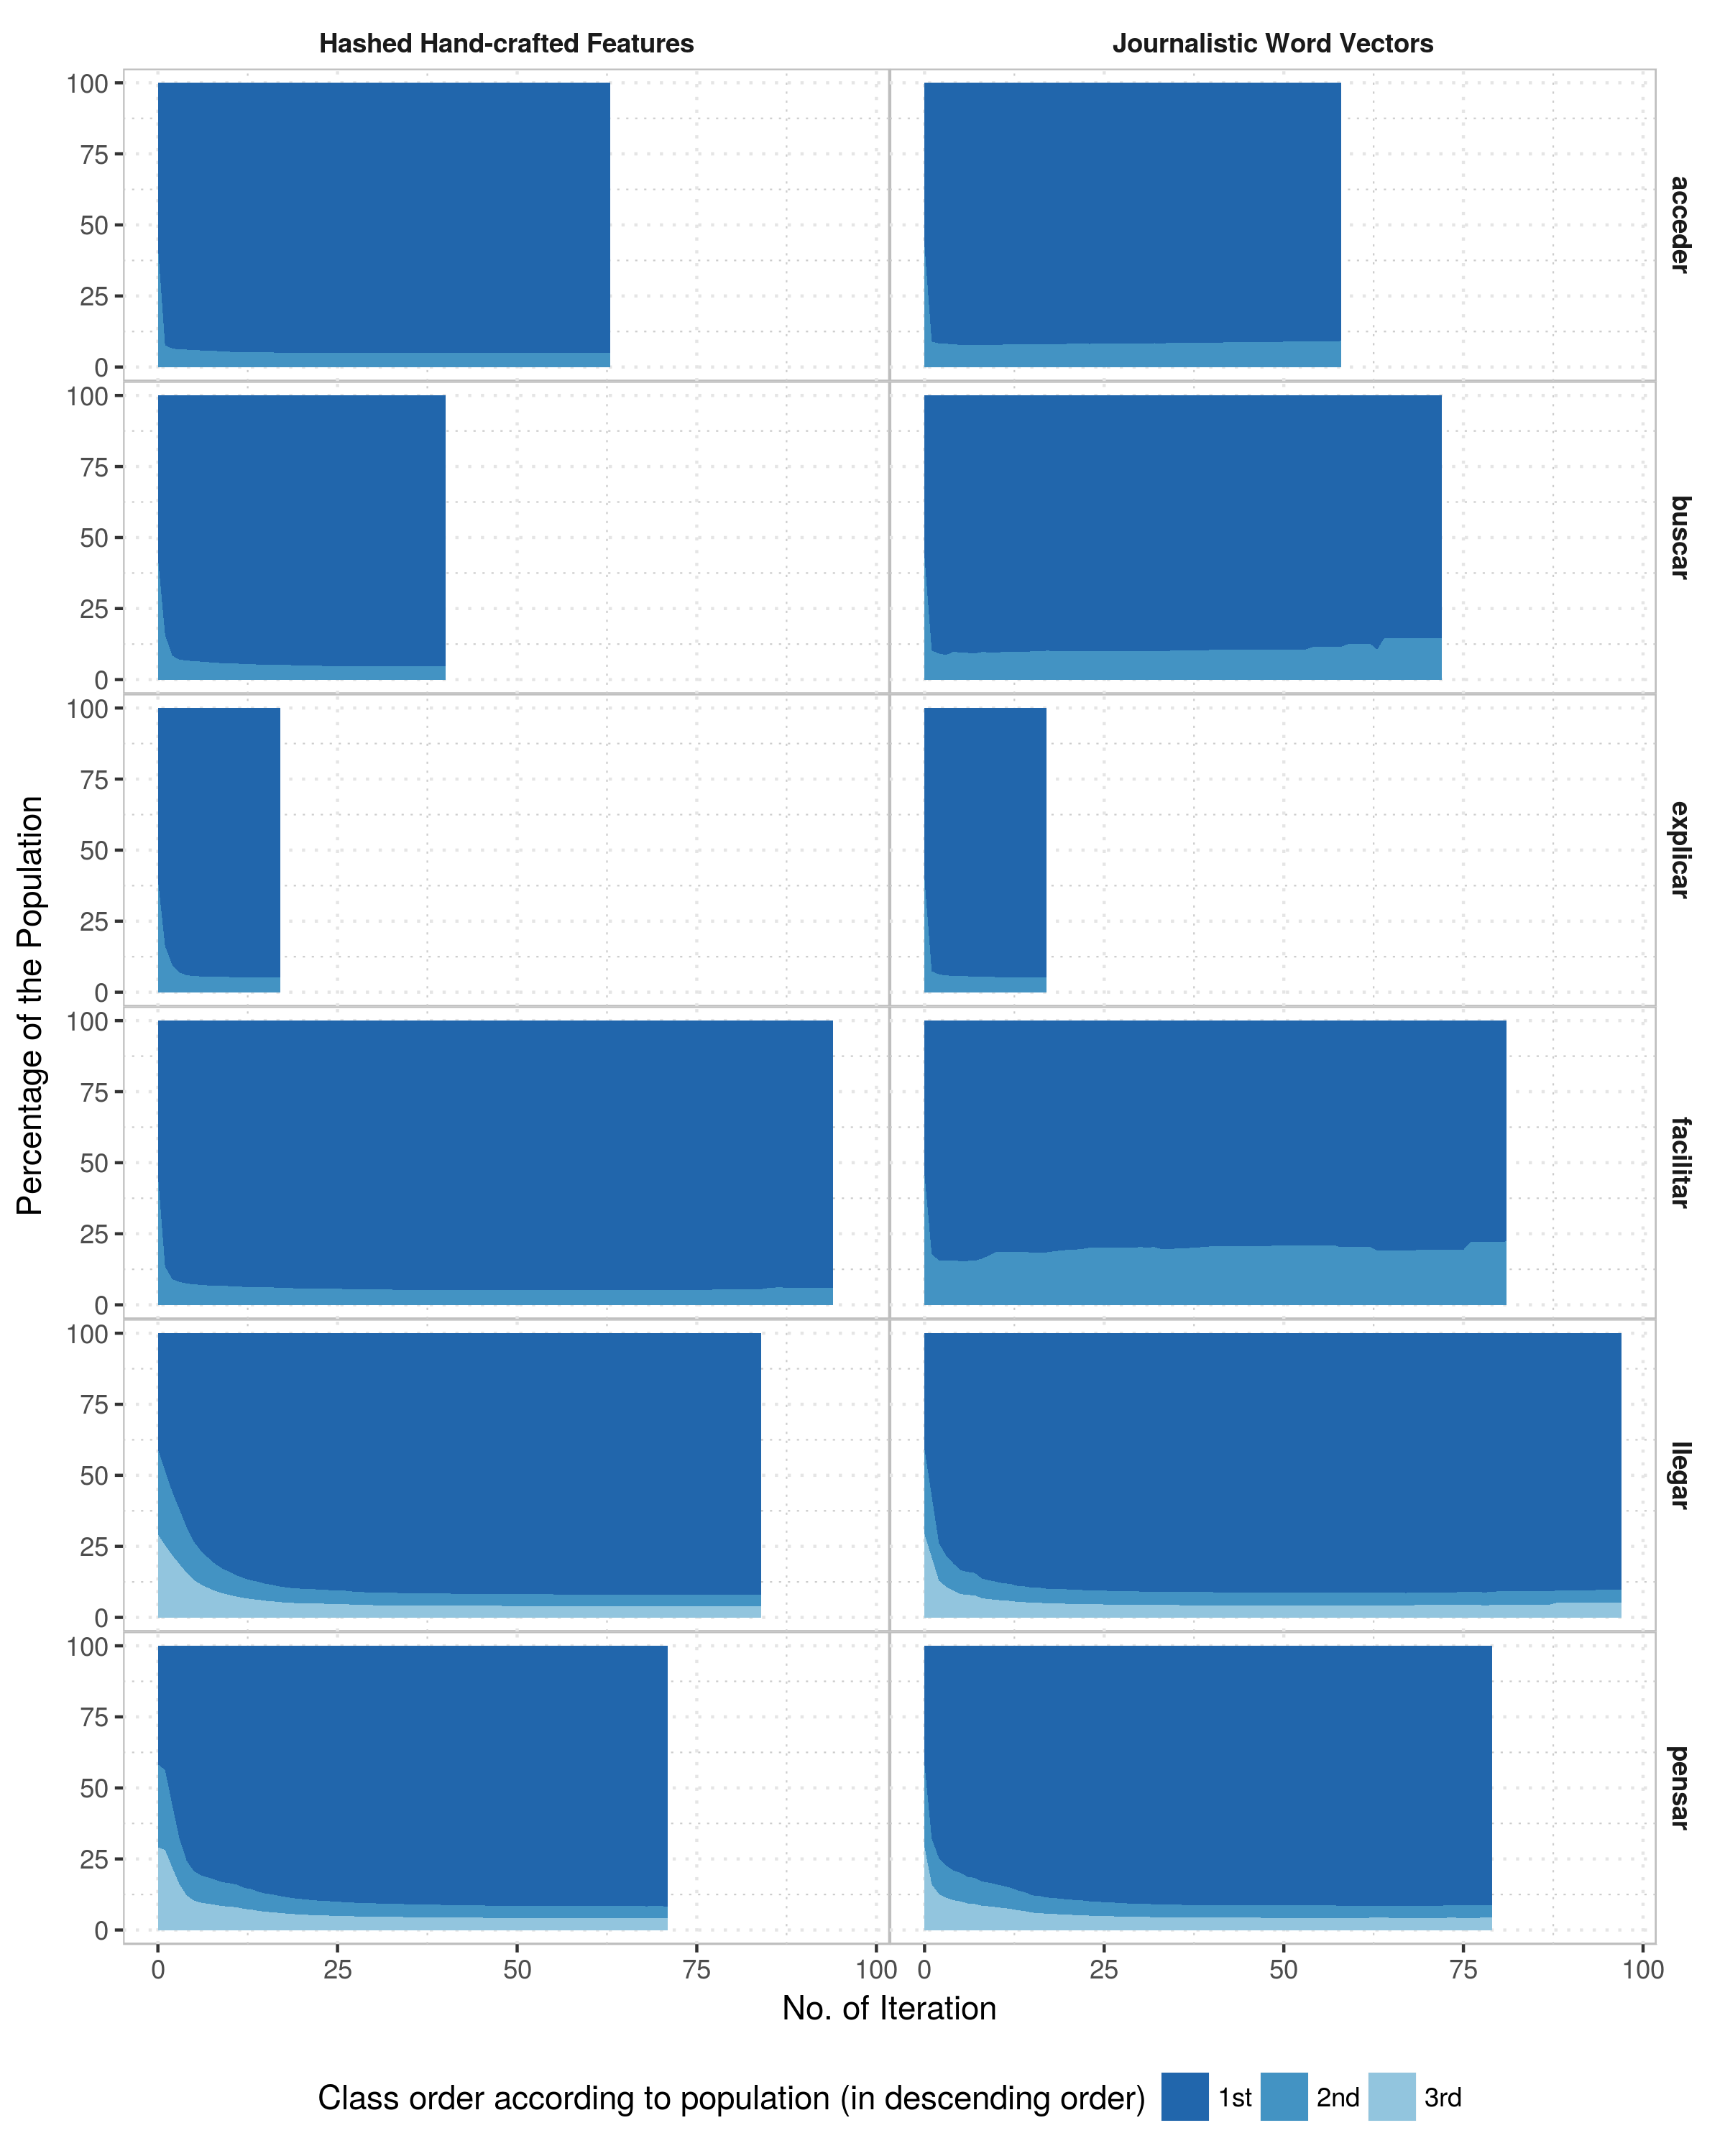
\includegraphics[height=.9\textheight,width=\textwidth,keepaspectratio]
    {plots/selflearning/population_distribution}
  \caption{Distribution of the classes' population across self-learning
  algorithm's iteration as a proportion of the whole training dataset}
  \label{fig:self-learning:population_distribution}
\end{figure}

Figure \ref{fig:self-learning:population_distribution} showcases the
distribution of the population of the classes across the self-learning
iterations of the algorithm. Each class's population is represented as the
proportion of the total number of examples in the training dataset for that
iteration. The plot is a stacked area plot that follows this structure:

\begin{itemize}
  \item Each row shows the results for a token lemma: ``acceder'', ``buscar'',
    ``explicar'', ``facilitar'', ``llegar'', and ``pensar''.
  \item Each column stands for a feature representation: hand-crafted hashed
    features and journalistic word vectors.
  \item The x-coordinate represents the iteration in the self-learning
    algorithm.
  \item The y-coordinate represents the percentage of population.
  \item Each area of a different color represents the proportion of examples
    for each of the classes in the dataset. The classes again are ordered
    according to number of examples in the original supervised dataset.
\end{itemize}

Figure \ref{fig:self-learning:population_distribution} shows the clear
predominance of the most frequent class in the self-learning algorithm. For
some lemmas the progress is a little less steep, for others the algorithm
starts to classify most instances into the most frequent class from the
beginning.

Recall that the number of classes is very unbalanced in the original manually
annotated corpus. To make this less of a problem, the corpus I have been using
in all these experiments has minority classes oversampled so that the number of
examples per class is more uniformly distributed. Even so, the models still
diverge quickly to the majority class.

From this figure I have evidence to reject the hypothesis regarding the
classes' distribution being uniform across the self learning iterations. This
figure gives me insight on that. However, to see more clearly what happens with
the classes on a per iteration basis the following visualization provides a
better view of the data.

\subsubsection{Population added per sense per iteration}

\begin{figure}[htb!]
  \centering
  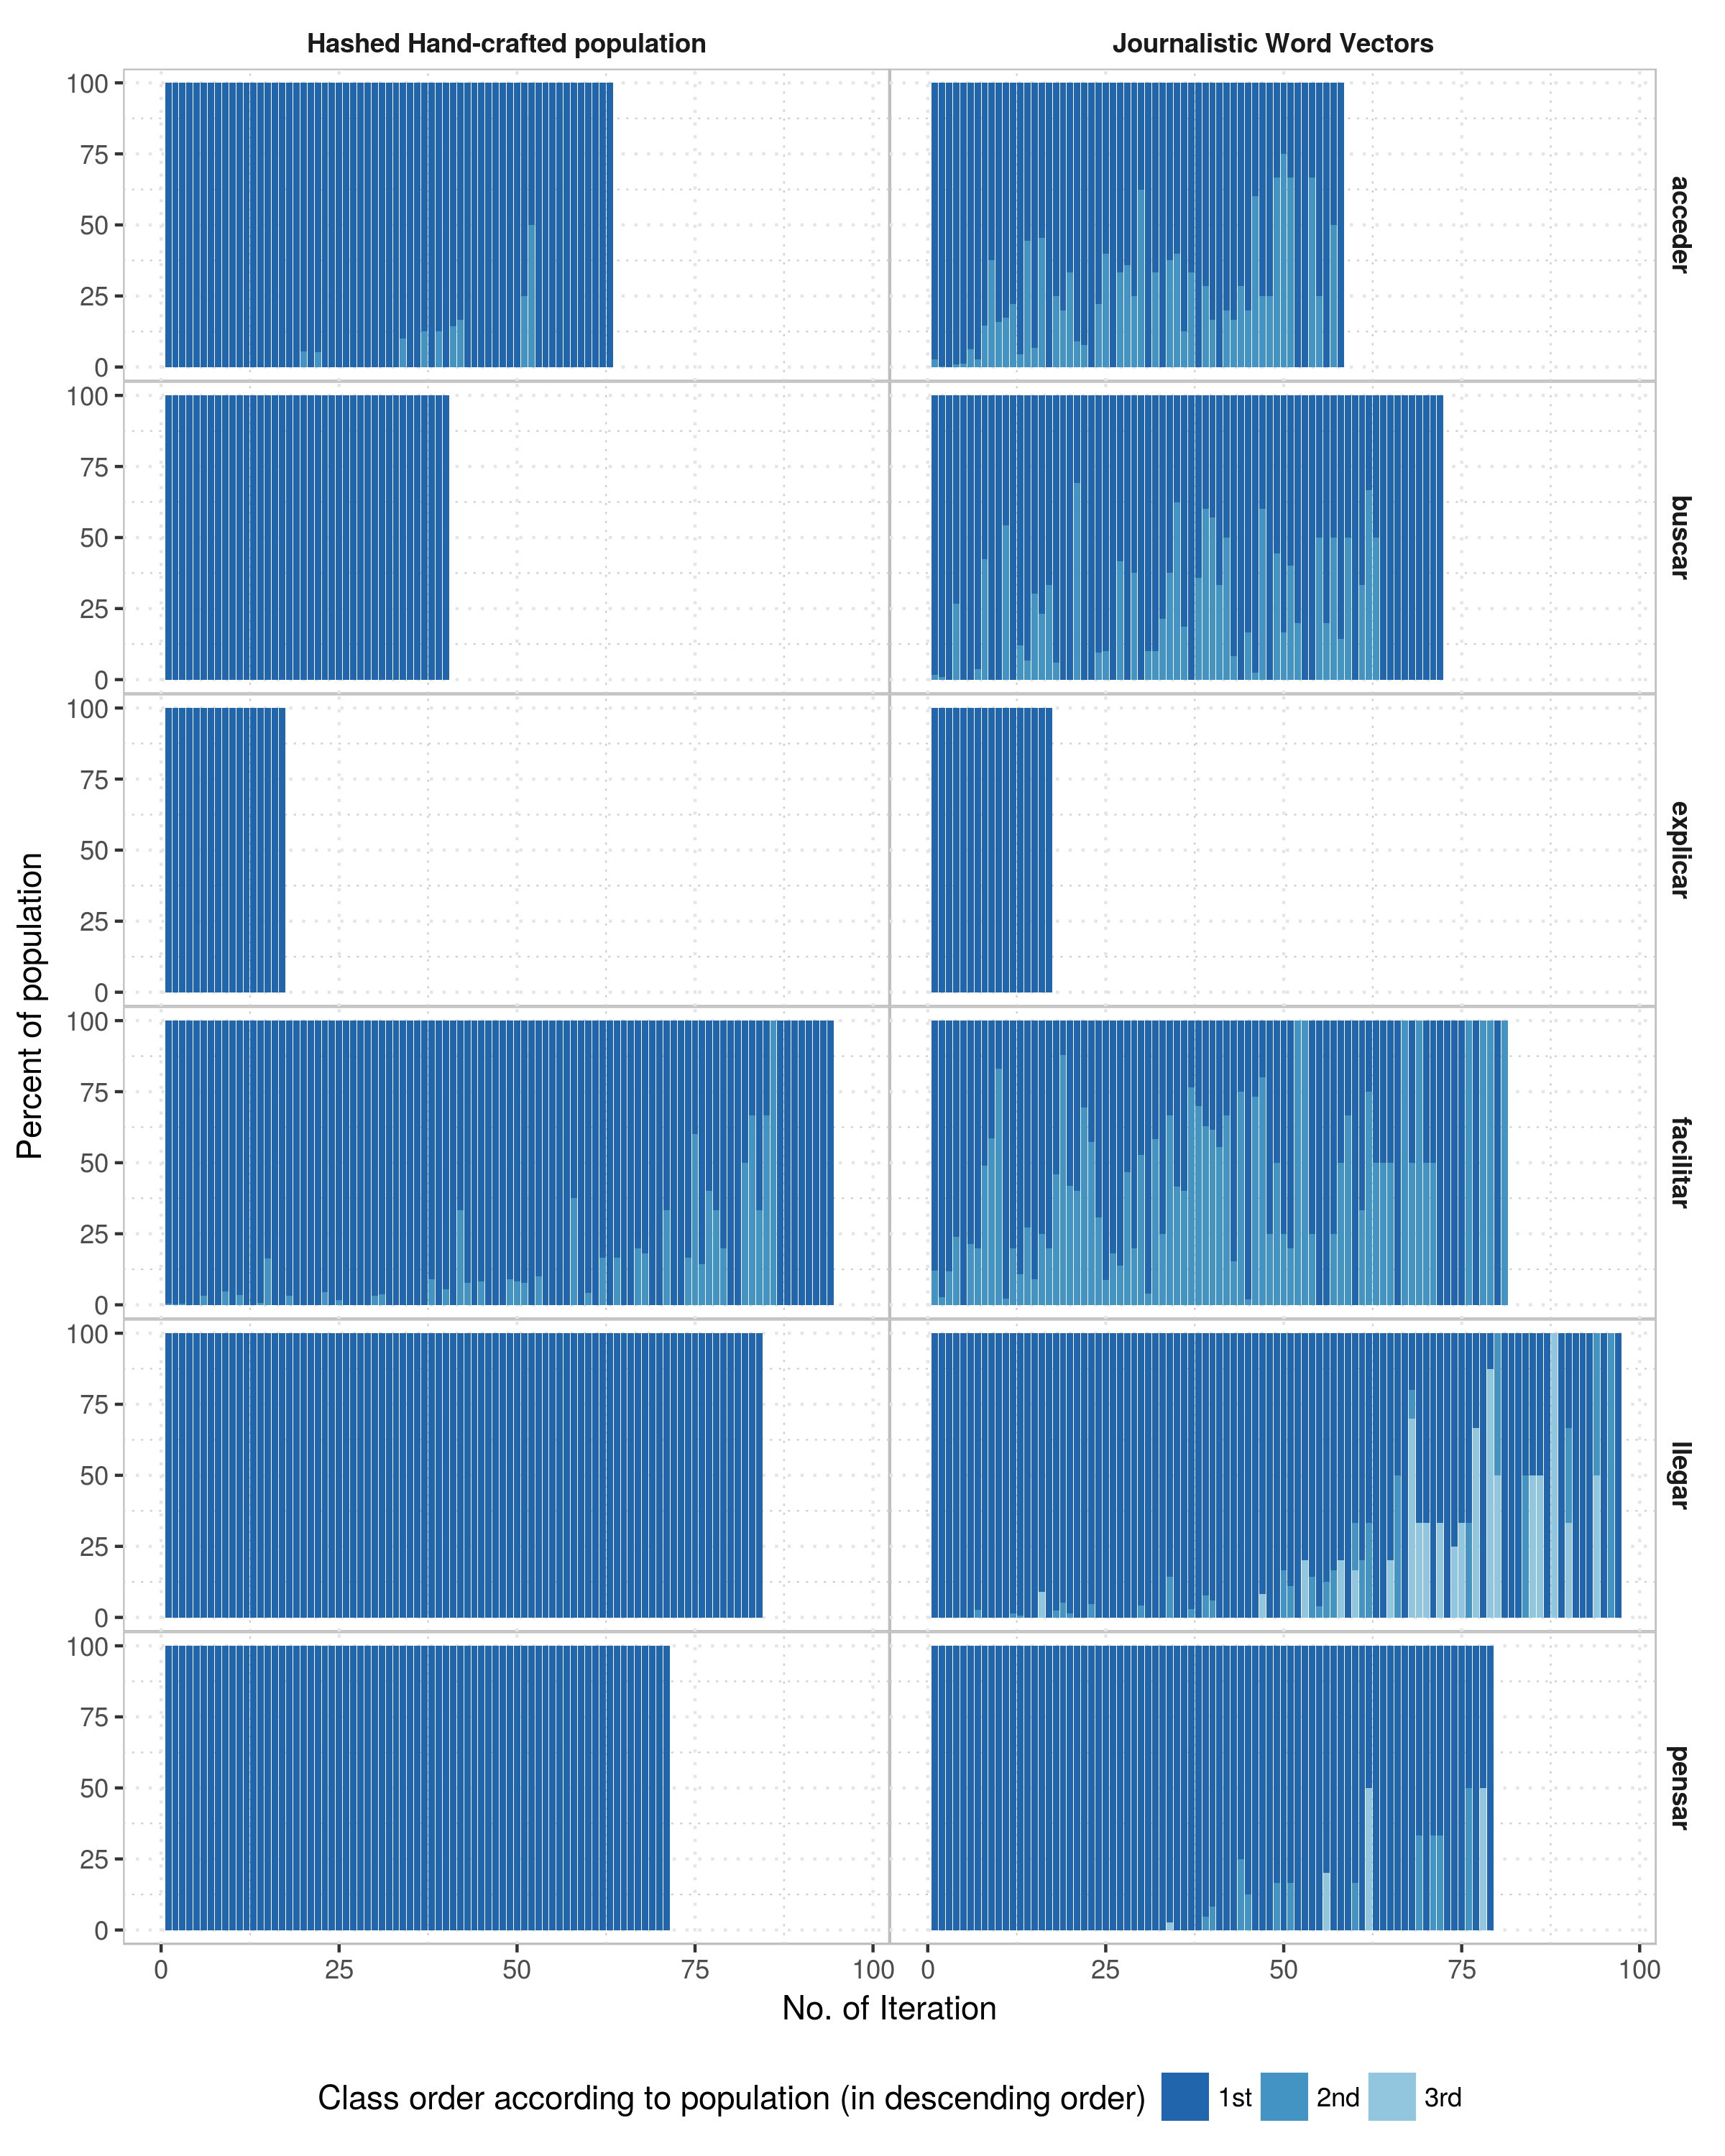
\includegraphics[height=.9\textheight,width=\textwidth,keepaspectratio]
    {plots/selflearning/population_add_per_class}
  \caption{Population added per sense on each iteration of self-learning as a
  proportional count of all the examples added in that iteration}
  \label{fig:self-learning:population_add_per_class}
\end{figure}

Figure \ref{fig:self-learning:population_add_per_class} shows the proportion of
examples added per class on each iteration. It is a stacked bar plot where each
bar represents the total examples added in the iteration, and each color in the
bar represents the proportion of classes automatically annotated as such. The
structure of the plot is the following:

\begin{itemize}
  \item Each row shows the results for a token lemma: ``acceder'', ``buscar'',
    ``explicar'', ``facilitar'', ``llegar'', and ``pensar''.
  \item Each column stands for a feature representation: hand-crafted hashed
    features and journalistic word vectors.
  \item The x-coordinate represents the iteration in the self-learning
    algorithm.
  \item The y-coordinate represents the percentage of examples automatically
    annotated and added to the model.
  \item Each bar plot represents the distribution of the examples added in the
    iteration. Each color of the stacked bar represents the class into which
    the examples were annotated.
\end{itemize}

This figure gives a better insight of what is happening on each iteration of
the algorithm and helps explain the distribution shown on Figure
\ref{fig:self-learning:population_distribution}, as it shows the proportion of
classes added in each iteration of each class.

I am able to see that the model trained with hand-crafted features practically
does not label the unlabeled data as something that is not the most frequent
class. This adds up to what is shown in previous paragraphs regarding
hand-crafted features having problems generalizing well to other domains.

The representation with word embeddings on the other hand is also affected, as
I saw in the previous figure, with the model diverging to the most frequent
class. However, there is a clear tendency for the model to also annotate
classes other than the most frequent one in the examples. And as I discussed in
Section \ref{sec:self-learning:hyp:1} the results of the self-learning
algorithm using word embeddings were quite superior to the ones obtained for
hand-crafted features. This means the word embeddings have a good impact on a
self-learning model as they help the classifier generalize better thus being
able to add new examples, even from different domains, to the model.

From this and the previous analysis I can conclude Hypothesis
\ref{hyp:self-learning:6} is false. Clearly it does not happen that the
self-learning model is adding new data uniformly distributed across classes.
Nevertheless word embeddings do help the model to add relevant data and not
labeling everything as part of the most frequent class. This is an interesting
line of future work as a deeper analysis, perhaps with manual evaluation, to
see how well word embeddings are helping to classify examples as part of the
less frequent classes.

\subsection{Hypothesis \ref{hyp:self-learning:7}}\label{sec:self-learning:hyp:7}

The last hypothesis I wanted to reject in this chapter is Hypothesis
\ref{hyp:self-learning:7}. The hypothesis states that the coverage given by the
features is uniform across classes. Recall that I showed in Section
\ref{sec:self-learning:hyp:4} that the number of features grew across
iterations of the self-learning algorithm, this was stated by Hypothesis
\ref{hyp:self-learning:4}. The previous section showed that the number of
classes is not maintained uniformly across the self-learning iterations, thus
it is natural to think this will happen with features as well. However, the
results I will show in this part are useful to throw some more light on the
results of the previous sections.

To test this hypothesis I want to measure two things: the raw count of the
features for each of the classes, and how strongly a feature is associated to a
class based on the pointwise mutual information it has with that class. These
results are obtained from Experiment \ref{exp:self-learning:4} which reports
the number of times a feature occurs with a class in the training dataset for
each iteration of the self-learning algorithm. To reduce the noise in the data
I filtered out all the pairs of $(features, classes)$ that co-occur less than 2
times.

\subsubsection{Features raw count}

The first view of the data I want to show is what comes to measure the results
of Experiment \ref{exp:self-learning:4} using the raw count. This shows the
number of unique features occurring with each class in each iteration of the
self-learning algorithm. In this view of the results, features can be present
in two classes at the same time, if they occurred more than twice with that
class, regardless of how strongly associated they are with the class.

\begin{figure}[htb!]
  \centering
  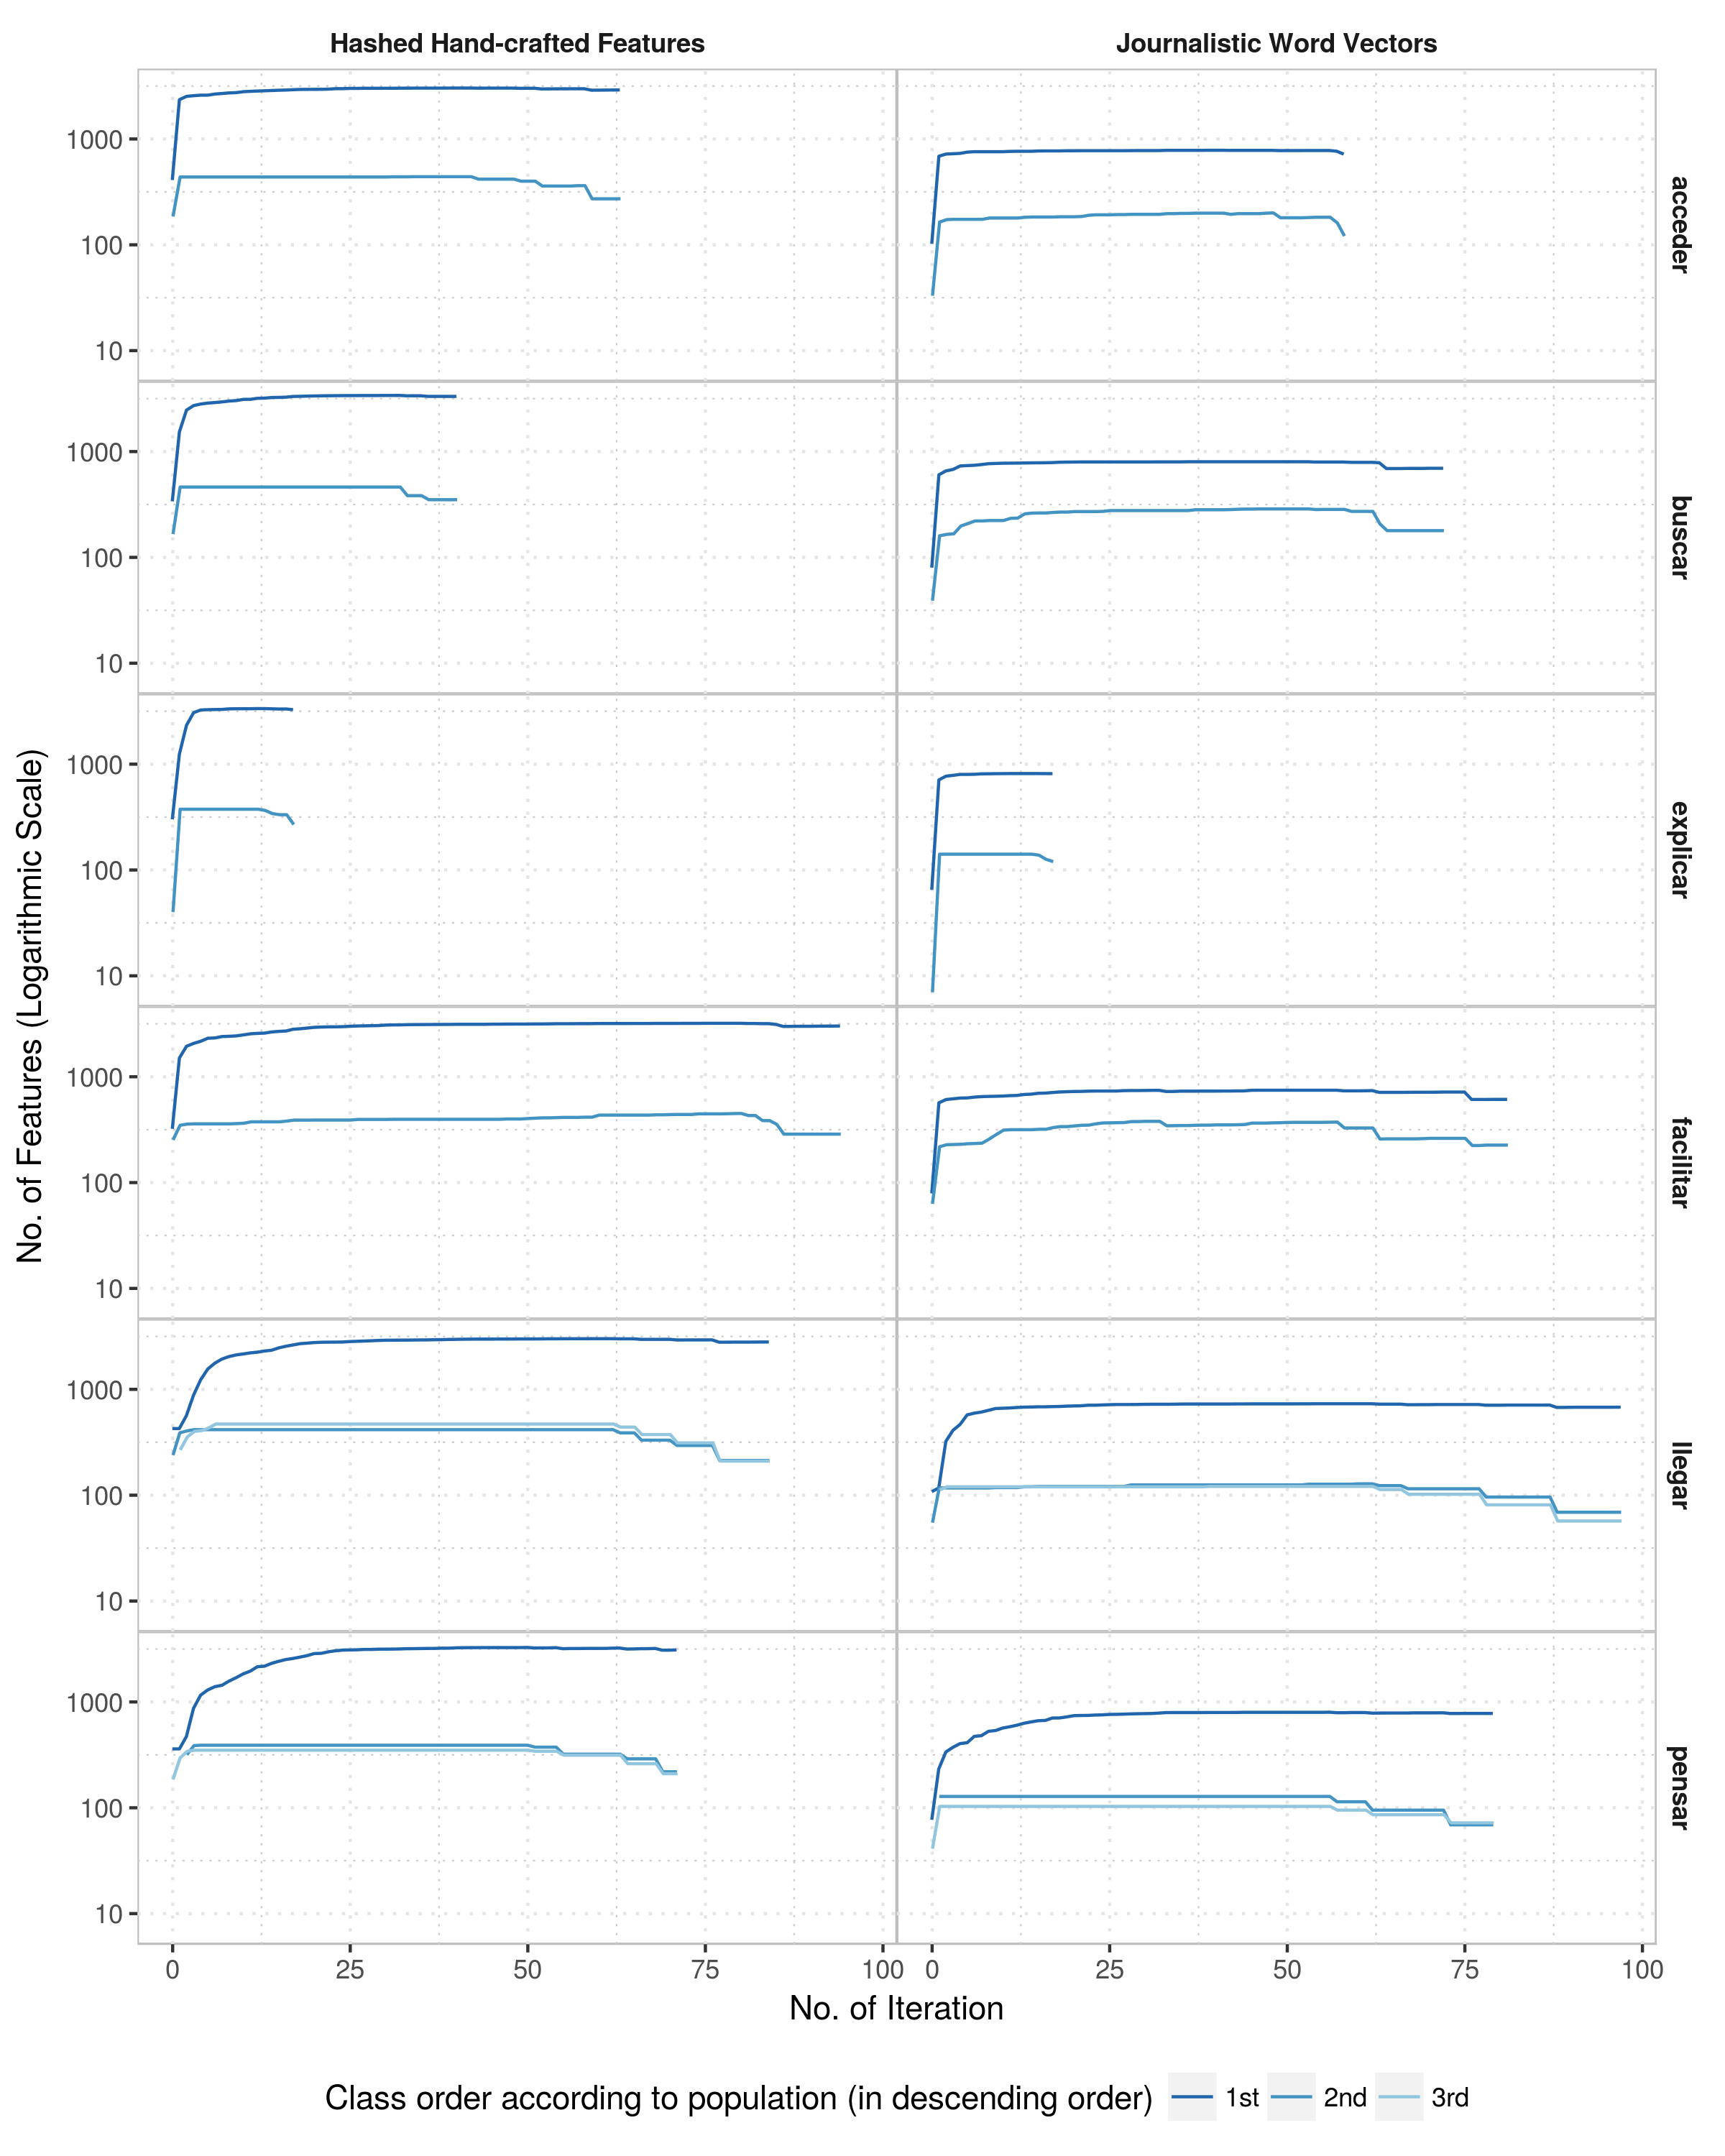
\includegraphics[height=.9\textheight,width=\textwidth,keepaspectratio]
    {plots/selflearning/features_growth_per_class}
  \caption{Features growth per class across self-learning iterations (in
  logarithmic scale)}
  \label{fig:self-learning:features_growth_per_class}
\end{figure}

Figure \ref{fig:self-learning:features_growth_per_class} displays the results
of counting the different features occurring with each of the classes in the
datasets. That is the total number of unique features up to that iteration
obtained both from the original supervised dataset and the automatically
annotated data. The figure shows a line plot with the following structure:

\begin{itemize}
  \item Each row shows the results for a token lemma: ``acceder'', ``buscar'',
    ``explicar'', ``facilitar'', ``llegar'', and ``pensar''.
  \item Each column stands for a feature representation: hand-crafted hashed
    features and journalistic word vectors.
  \item The x-coordinate axis represents the iteration number in the
    self-learning algorithm.
  \item The y-coordinate axis represents the raw count of unique features in a
    logarithmic scale. The scale selected is logarithm because, in comparison,
    the number of features of the most frequent class is an order of magnitude
    larger than those of the less frequent classes, and any variation (i.e.
    adding more features) of the less frequent classes is lost when compared to
    the most frequent class if I use a linear scale.
  \item Each line represents the number of features and the different colors
    represents the class that features belong to.
\end{itemize}

The figure shows that there is always a class for which the number of features
increases much more quickly and in a higher number than the others. This is a
consequence of the model diverging to the most frequent class. Most of the new
features also come from the first iterations of the algorithm and in the
following ones there are practically no more new features added. This is
particularly noticeable for the less frequent classes. As a consequence of
this, after some initial few iterations the algorithm diverges and all new
instances are directly added to the most frequent class. Thus in the last
iterations of the algorithm there are not new features for the less frequent
classes.

Once again the difference between hand-crafted features and word embeddings
resides in the pool of features. As I explained previously, the pool of
features that comprise the word embeddings model is much smaller than for
hand-crafted features. Nevertheless it is interesting that in some of the
lemmas the features grow for each class in the latter iterations for word
embeddings, while it does not for hand-crafted features. This comes from what I
saw in the previous Section regarding word embeddings helping the model
generalize better and annotate new classes besides the most frequent one.

There is an effective increase in the coverage, as many features are added to
the model. However these features belong mostly to a single class, the majority
class. In the following section I will show that this increase in the number
of features does not directly imply an improvement of the model.

\subsubsection{Features PMI}\label{sec:self-learning:featurespmi}

The second view of the data I want to show is based in the results of the
experiment measuring the correlatedness between features and classes. This is
given by the pointwise mutual information (PMI) between the features and the
associated classes given by Metric \ref{met:4}.

\begin{figure}[htb!]
  \centering
  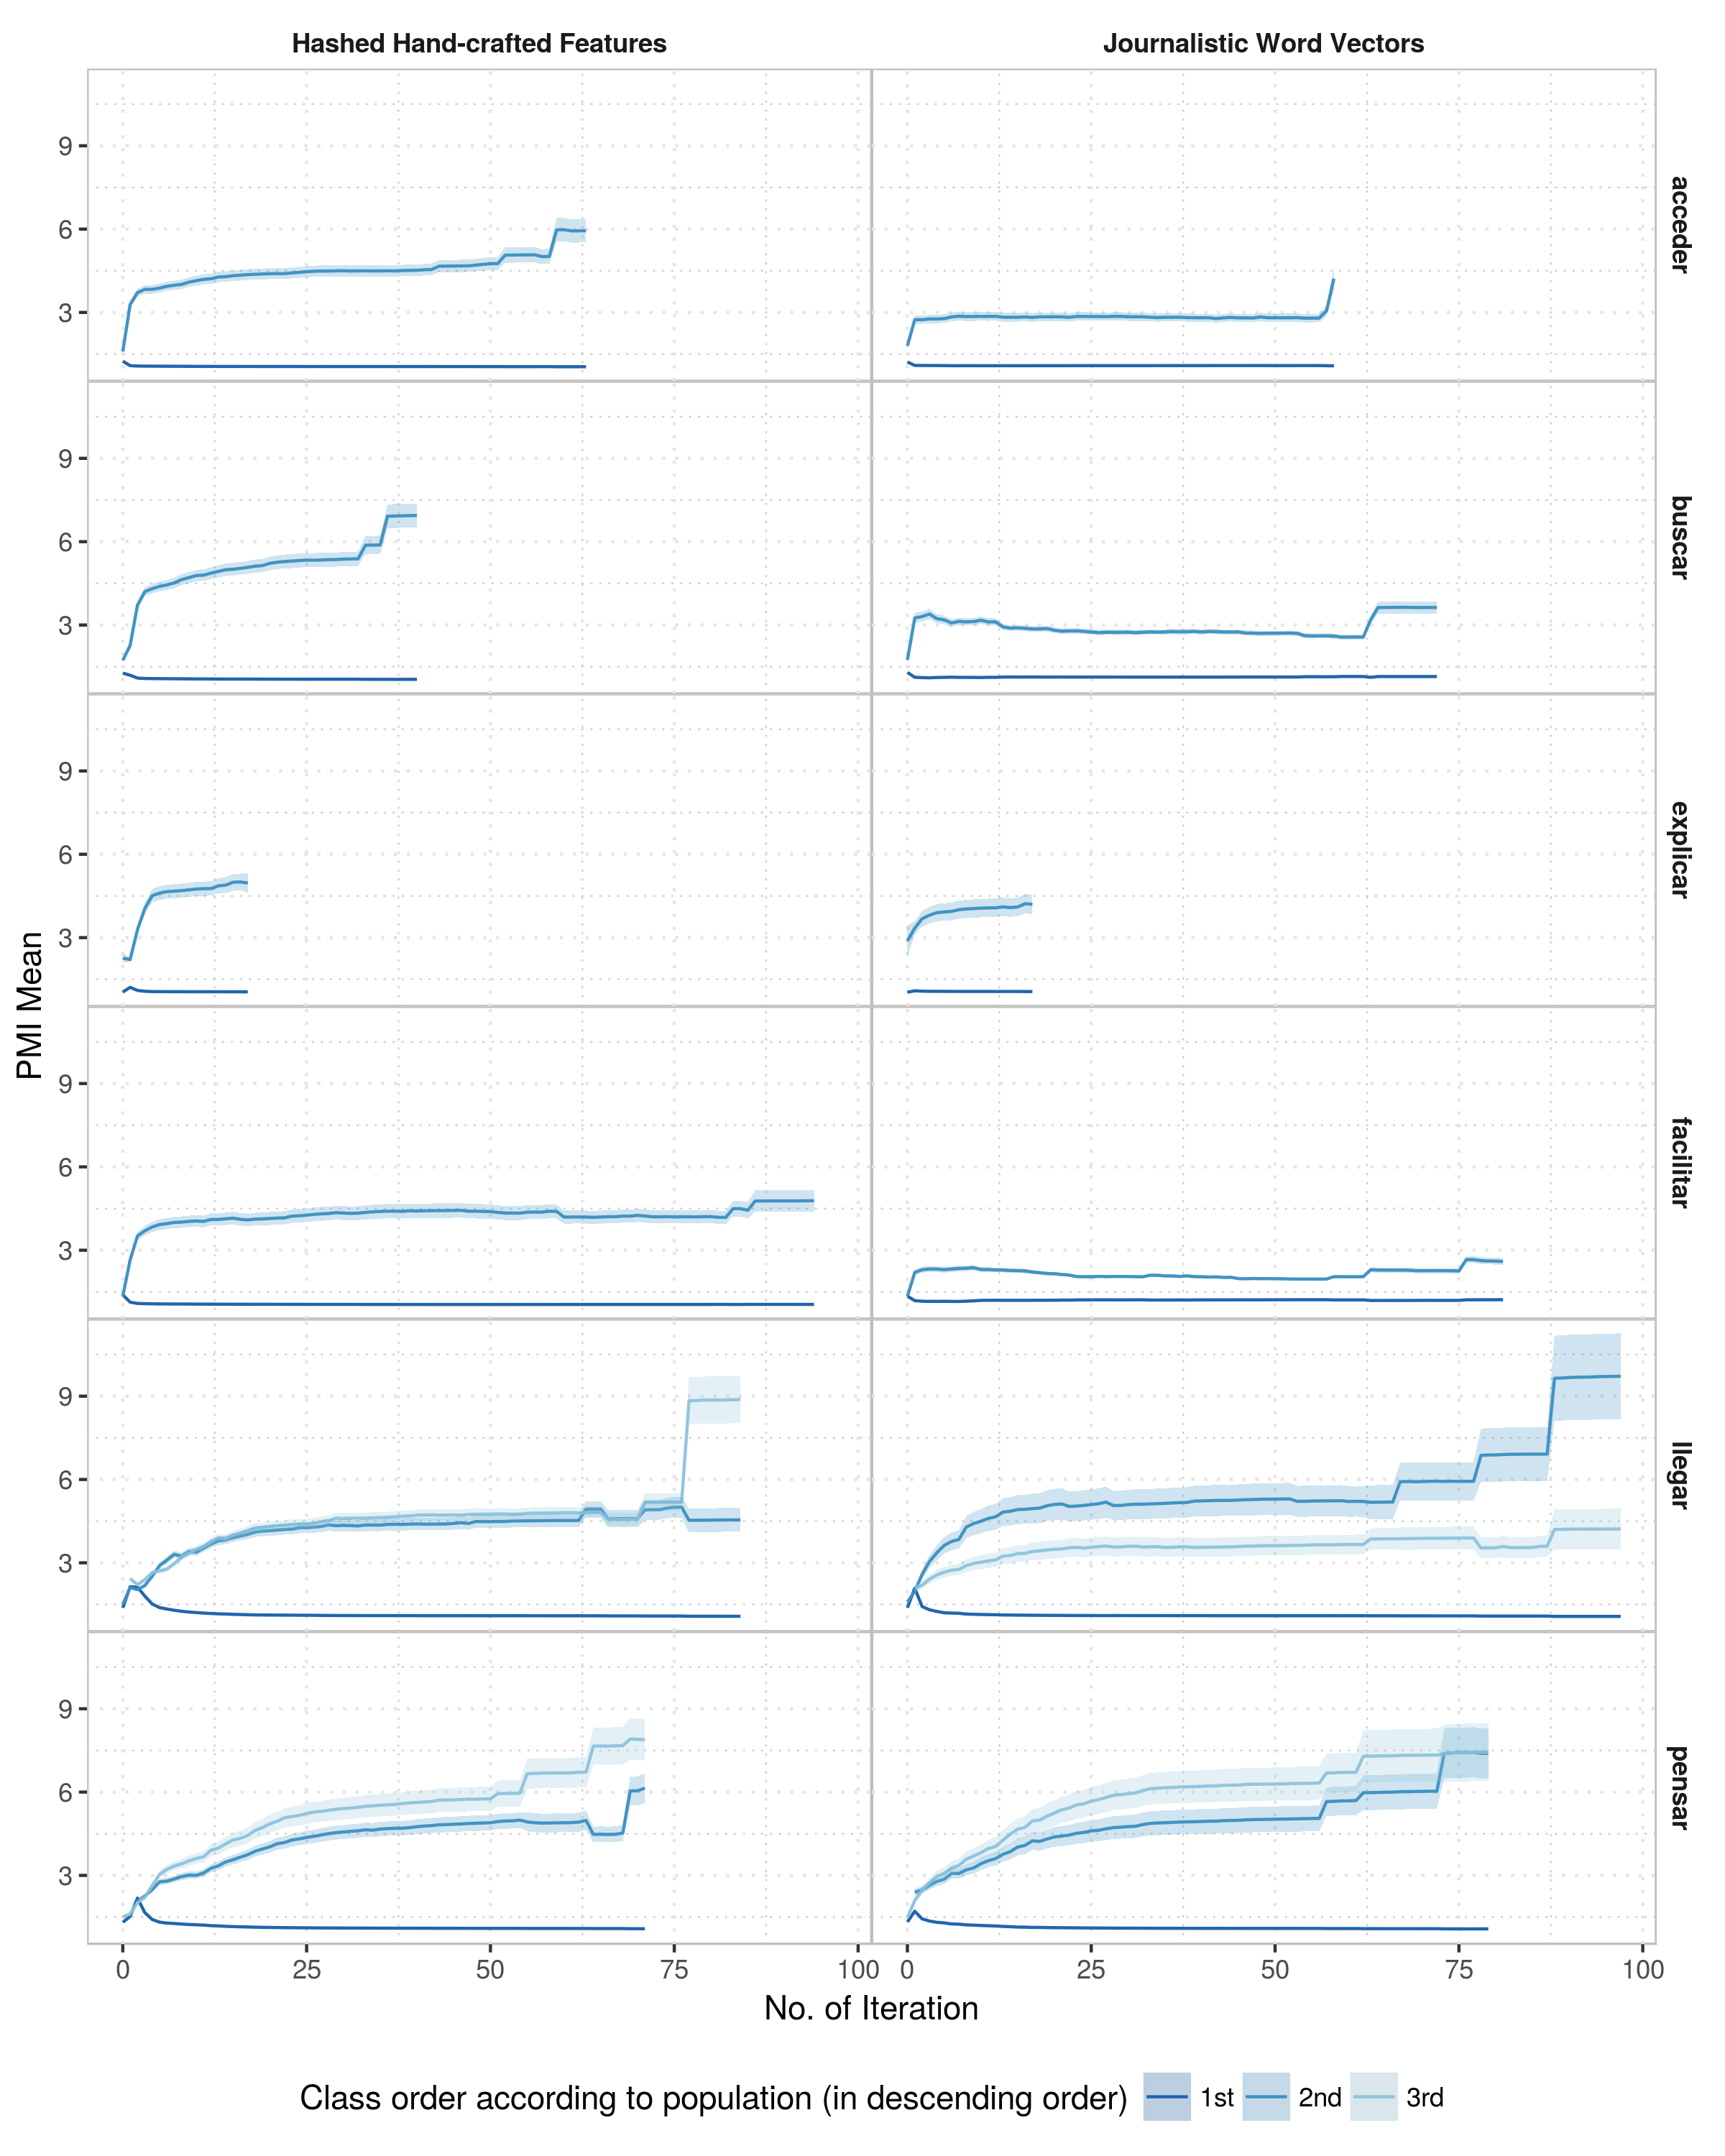
\includegraphics[height=.9\textheight,width=\textwidth,keepaspectratio]
    {plots/selflearning/features_pmi}
  \caption{Features pointwise mutual information with each of the classes
  across self-learning iterations}
  \label{fig:self-learning:pmi}
\end{figure}

Figure \ref{fig:self-learning:pmi} displays the mean and standard error of the
mean of the pointwise mutual information between features and classes across
the self-learning iterations. Thus it is higher when the features associated to
a class are associated more strongly to the class. Recall that the metric
associates each feature to the class it has a higher PMI with. The figure shows
a line plot with the following structure:

\begin{itemize}
  \item Each row shows the results for a token lemma: ``acceder'', ``buscar'',
    ``explicar'', ``facilitar'', ``llegar'', and ``pensar''.
  \item Each column stands for a feature representation: hand-crafted hashed
    features and journalistic word vectors.
  \item The x-coordinate axis represents the iteration number in the
    self-learning algorithm.
  \item The y-coordinate axis represents the raw count of unique features in a
    logarithmic scale.
  \item Each color represents a class.
  \item The line of darker color in the middle represents the mean of the PMI
    for the class and the shadowed area represents the standard error of the
    mean for that PMI.
\end{itemize}

Different from the previous figure, now the classes with a smaller number of
features are the ones having the larger values in the plot. It seems that in
classes with a smaller number of features, these are associated more strongly
to the class. In contrast, in classes with a bigger number of features, these
are associated more weakly. It seems that the most frequent class is working as
a ``catch all'' for new examples, mostly those without features strongly
associated to any other class, and because of the algorithm's tendency to
annotate examples to it. Then, the features in these new examples are
associated to that class. However, these features are not strongly related to
that class, because they belong to examples that have been classified into the
class by weak reasons, like the probability of the class or the lack of
characterizing features. This makes these features not a good parameter to help
discriminate this class. On the other hand the features for the less frequent
classes become much more discriminative of such classes because new examples
are only classified into those classes when there is strong evidence that they
belong to the class, that is, when evidence is stronger than the default to
classify them into the majority class.

Even if it looks like the classifier's coverage is increasing, because of the
number of features doing so, from this data there is a clear indication that it
is not like that because the new features belong mostly to the most frequent
class and do no contribute to increase the certainty of the model, which is
reflected on a low mean of the PMI with the most frequent class.

On the other hand, those features that are associated to the less frequent
classes do so with a strong association to the point that as the self-learning
iterations add new examples the features become more discriminative of this
less frequent classes. However, the number of these features does not increase
as much, as was shown in the previous section.

\subsection{Summary}

The results of the evolution of certainty and tendency to overfit in the model
give the impression that hand-crafted features have less variance than word
embeddings. However, a more detailed analysis shows that even though the
variability is less in hand-crafted features, the reason behind this is that it
only adds new examples of a particular class, the most frequent one. This is
not the case for word embeddings.

Word embeddings show more variability in the tendency to overfit and the mean
of the certainty as it is effectively adding new examples annotated into
classes that are not only the most frequent one. Moreover, Figure
\ref{fig:self-learning:population_add_per_class} shows there are some instances
where only elements of the less frequent classes are added.

\section{Conclusions}\label{sec:self-learning:conclusions}

In this chapter I have presented an approximation to self-learning to overcome
the problems of overfitting and coverage presented in the previous chapters.
My initial hypothesis was that the overfit is caused by the low number of
examples and that increasing such number helps reducing it.

I saw that adding new examples effectively helps reducing the overfit in the
initial iterations. However, self-learning is biased to the most frequent
class. This makes the model add many examples to that class, ignoring the less
frequent classes. This is particularly noticeable for hand-crafted features.

To draw this conclusion I defined some subhypotheses in the beginning of the
chapter. The experiments done to test these hypotheses gave me the possibility
to draw the following conclusions.

Hypothesis \ref{hyp:self-learning:1} that the performance of the model over a
held-out test dataset improves after the self-learning algorithm was shown
false for the case of hand-crafted features but I could not obtain conclusive
results to reject it with respect to word embeddings. In the latter case the
results depended on the lemma, as for some the performance decreased but for
others it increases or remains the same. An important results I could gather
from this is that hand-crafted features had a steeper drop in performance than
word embeddings, a sign that the representation fits the labeled dataset well
but fails to generalize.

Hypothesis \ref{hyp:self-learning:2}, which stated that the model's average
certainty on unseen examples in each iteration is increased, is rejected in
light of the obtained results. This is because there is a clear tendency of
the certainty of the mean that the algorithm has over unseen data to decrease
across iterations. 

Hypothesis \ref{hyp:self-learning:3}, which states that overfitting is reduced
across self-learning iterations, is mildly rejected. The fact is that the
number of examples effectively reduced overfitting in the first iterations of
the algorithm. However, as I do not use this as a stopping criterion in the
algorithm, when it starts to diverge to the most frequent class, the tendency
to overfit increases.

Hypothesis \ref{hyp:self-learning:4} stated that the coverage of the model
increases as a result of increasing the number of features associated to this
model. The number of features associated to the model indeed increases as the
results did show. These results are enough to accept the stated hypothesis.
However, as I saw in the results associated to Hypothesis
\ref{hyp:self-learning:7}, which conclusions are in the next paragraphs, these
results are not enough to show that there is an indication of the model
effectively increasing coverage as a result of increasing the number of
examples.

The previous hypotheses were formulated with the idea to accept them. This was
not exactly the case. However, the other three hypotheses in this chapter were
formulated with the idea they would be rejected.

Hypothesis \ref{hyp:self-learning:5} states that the performance of the
self-learning algorithm over all the classes is improved. The hypothesis is
rejected because only the performance of the most frequent class increases
through iterations of the self-learning algorithm, while the rest of the
classes show a degraded performance.

Hypothesis \ref{hyp:self-learning:6} states that the representativity of each
class in the dataset is kept through all the iterations of the algorithm. The
hypothesis is also rejected. The results show that new examples added to the
model belong mostly to the most frequent class and the distribution of the
classes is highly biased across the iterations. In particular, hand-crafted
features have the worst performance in this as the model only adds examples of
the most frequent class. Word embeddings have better performance as the
algorithm adds examples of the less frequent classes as well. This last has
relation to what happens in the results of the previous hypothesis where there
are some cases where the less frequent classes' performance does not drop to
zero as in hand-crafted features.

Hypothesis \ref{hyp:self-learning:7} states that the coverage of the features
is uniformly distributed across the classes. The results obtained serve to
prove the hypothesis false. This hypothesis is related to Hypothesis
\ref{hyp:self-learning:4} which states that the number of features associated
to the model increases after the self-learning iterations, which is true, but
not in the way the model needs in order to effectively increment the coverage.
This is because the certainty of the model does not increase with the number of
features. In a detailed analysis it is seen that most of the features are
weakly associated to the classes (in particular to the most frequent class).
So, their contribution to the model is small. Thus a bigger number of features
does not imply a better model, not even better coverage, because they are not
discriminative enough. A possible cause of this is that, when the model starts
to overfit, the most frequent class begins to coopt elements that are not part
of the class. This makes the model drift and starts to have less certainty over
new examples.

As I saw in the results of this chapter, the biggest problem for self-learning
is the tendency to diverge and add everything to the most frequent class. A
way of attacking this problem is using techniques which help stop that bias.
There are different ways to do so. One is by re-sampling the data. I only
explored random oversampling of the less frequent classes, which did not prove
useful. Other re-sampling methods include the random sub-sampling of the most
frequent class or a mix of both.

In the next chapter I will explore a technique based on human annotation which
selects examples based on high uncertainty and give that to a domain expert in
order to correctly annotate them. The idea is that this examples will help the
model better define the decision boundaries over the most frequent class, which
is something the self-learning algorithm is not doing well.

Future work of this chapter includes the change of the stopping criterion for
something to stop once the model becomes to overfit again (the spread between
training error and validation error grows). Another line of future work is a
more general analysis of all the lemmas, and some more specific analysis on
some more lemmas beside the selected tokens.

I also have to do more thorough analysis of the certainty the model has over
new examples (i.e. previously unseen) and why it becomes so irregular as the
algorithm's iterations go further.

Finally, as word embeddings proved to have interesting results and, unlike
hand-crafted features, they did not drift so quickly or so firmly to the most
frequent class, it would be interesting to do some manual evaluation and error
analysis to see what is happening under the hood.
